% !TEX root = ../Thesis.tex
\acresetall
\myChapter[Finite element \threed reconstruction of the pulmonary acinus]{Finite element \threed reconstruction of the pulmonary acinus imaged by synchrotron X-ray tomography}\label{ch:tsuda2008}

%\newcommand{\footremember}[2]{\footnote{#2}\newcounter{#1}\setcounter{#1}{\value{footnote}}}%
%\newcommand{\footrecall}[1]{\footnotemark[\value{#1}]} 

Akira Tsuda\footremember{boston}{School of Public Health, Harvard University, Boston, Massachusetts, USA}\textsuperscript{,}\footnote{Address for reprint requests and other correspondence: A. Tsuda, Molecular and Integrative Physiological Sciences, Harvard School of Public Health, 665 Huntington Ave., Boston, MA 02115 (e-mail: \href{mailto:atsuda@hsph.harvard.edu}{atsuda@hsph.harvard.edu}).}\\%
Nenad Filipovic\footnote{University of Kragujevac, Kragujevac, Serbia}\\%
David Haberthür\footremember{ana2}{Institute of Anatomy, University of Bern, Bern, Switzerland}\\%
Rene Dickie\footrecall{boston}\\%
Yasuto Matsui\footnote{Graduate School of Engineering, University of Kyoto, Kyoto, Japan}\\%
Marco Stampanoni\footnote{Swiss Light Source, Paul Scherrer Institut, Villigen, Switzerland}\\%
Johannes C. Schittny\footrecall{ana2}\\\\
First published in: J Appl Physiol 105: 964–976, 2008.\\
\href{http://dx.doi.org/doi:10.1152/japplphysiol.90546.2008}{doi:10.1152/japplphysiol.90546.2008}
\vfill
 \section{Abstract}
The alveolated structure of the pulmonary acinus plays a vital role in gas exchange function. Three-dimensional (\threed) analysis of the parenchymal region is fundamental to understanding this structure-function relationship, but only a limited number of attempts have been conducted in the past because of technical limitations. In this study, we developed a new image processing methodology based on \ac{fe} analysis for accurate \threed structural reconstruction of the gas exchange regions of the lung. Stereologically well characterized rat lung samples~\cite{Tschanz2003} were imaged using high-resolution synchrotron radiation-based X-ray tomographic microscopy. A stack of 1024 images (each slice: 1024$\times$1024 pixels) with resolution of \SI{1.4}{\micro\meter\cubed} per voxel were generated. For the development of \ac{fe} algorithm, multiple regions of interest, containing 7.5 million voxels, were further extracted as a working subunit. \threed \acp{fe} were created overlaying the voxel map using a grid-based hexahedral algorithm. A proper threshold value for appropriate segmentation was iteratively determined to match the calculated volume density of tissue to the stereologically determined value~\cite{Tschanz2003}. The resulting \threed \acp{fe} are ready to be used for \threed structural analysis as well as for subsequent \ac{fe} computational analyses like fluid dynamics and skeletonization.
\clearpage
\section{Introduction}
The mammalian interthoracic respiratory tract can be divided into two areas: conducting airways and pulmonary parenchyma (\ie, the gas exchange region of the lung). The conducting airways are a bifurcating network of relatively well-defined conduits carrying the ambient air to the parenchyma. Airways within the parenchyma---customarily called acinar/alveolar ducts---on the other hand, are not pipelike; they are formed by entrance rings of alveoli opening into a common passageway. Currently, enormous efforts (\eg, \cite{Aykac2003,Chaturvedi2005,Cheng2007,Chooi2004,Dame2006,Driehuys2007,Kvistedal2006,Ley2008,Scadeng2007,Sera2003,Tawhai2004,VanErtbruggen2005}) are devoted to reconstructing the conducting airway network in three dimensions (\threed), facilitated by rapid advancement of imaging technologies (\eg, \ac{uct}, hyperpolarized-gas \ac{mri} (\cf{HHe} 3 \ac{mri}, etc.), as well as a rapid increases in computing power.

In contrast to conducting airways, lung parenchyma is harder to access; the structures are physically small and located distally in the respiratory tract. Basic structures of lung parenchyma are highly complex; this complexity can be easily envisioned by the fact that the enormously large surface area of lung parenchyma, as large as that of a tennis court in the case of human lungs~\cite{Gehr1978,Weibel1963}, for example, has to be folded in within the lung cavity. At the same time, the image resolution required to obtain reasonable details of this complexity is on the order of a few micrometers [considering, for instance, the thickness of alveolar septa (inter-air space septa) of roughly \SI{10}{\micro\meter} (\cite{Gehr1978}; P. Gehr, personal communication)]. This required resolution is much finer than the resolution of commonly available \ac{mri} or even \ac{uct} mentioned above, but can be obtained with \ac{srxtm}.

Despite these difficulties, the motivations for reconstructing the \threed geometry of the respiratory region of the lung are numerous. Two-dimensional (\twod) sections of lung parenchyma are insufficient for many purposes and can produce erroneous models of lung structure~\cite{Cookson1993}. For instance, \threed structural rendering is crucial to the study of micromechanics in \threed acinar microarchitecture, particularly given the likelihood of heterogeneous behavior with ventilation. Only by using a realistic \threed structure (for example, of alveolar shape and orientation of the alveolar opening with respect to the central thoroughfare acinar channel) can the qualitative and quantitative effects of \threed acinar geometry on gas and aerosol transport be determined. Despite the necessity of accurate \threed structural renderings of the gas exchange regions of the lung, there have been only a handful of attempts in the past (\eg., \cite{Berend1991,Cookson1993,Honda2002,Litzlbauer2006,Mercer1987,Mercer1987a,Randell1989,Stelter1966,Watz2005}), mainly because formidable effort was required using traditional specimen preparation and imaging techniques.

Here we present our new effort at \threed reconstruction of the acinar air space in fixed lung tissue using the novel technology of \ac{srxtm} and subsequent \threed modeling of the obtained images. Because of the large specimen volume that can be imaged at high resolution using this method, we anticipate that it will ultimately allow \threed reconstruction of the entire air space of one acinus. Such a detailed rendering and consequent \threed quantitative analysis of structural measures of acinar morphology will prove invaluable to many studies, including performing the computational fluid dynamics of aerosol deposition in the gas exchanging areas of the lung. In this paper, we demonstrate the ability of \ac{srxtm} to render greater volumes ($10^9$~\micro\meter$^3$) of lung tissue than is possible by confocal microscopy and to achieve greater resolution (voxel size=\SI{1.4}{\micro\meter\cubed}) than possible by traditional \ac{uct}. We describe state-of-the-art \acf{fe} technology for \threed reconstruction of both tissue and air spaces in the acinus in detail; the outcome would be ready for subsequent \ac{fe} computational analyses like fluid dynamics and skeletonization.

\renewcommand{\imsize}{\linewidth}
\begin{figure}%[h]
	\centering
	\begin{tikzpicture}[,auto,%
		decision/.style={diamond, draw, thick, text width=5em, text centered},%
		block/.style ={rectangle, draw, thick, text width=13em, text centered, rounded corners, minimum height=2.5em},%
		line/.style ={draw, thick, -latex',shorten >=0pt}]
		\matrix [column sep=10mm, row sep=5mm]
			{
			& \node [block] (prep) {Tissue Preparation}; & \coordinate (dummy-prep);\\
			& \node [block] (sync) {Synchrotron Imaging}; & \coordinate (dummy-sync);\\
			& \node [block] (3d) {Preparation of \threed images from the original \twod slices}; & \coordinate (dummy-3d);\\
			& \node [block] (seg) {Segmentation technique}; & \coordinate (dummy-seg);\\
			& \node [block] (oca) {\acl{oca}}; & \coordinate (dummy-oca);\\
			& \node [block] (rec) {\threed reconstruction of separated objects}; & \coordinate (dummy-rec);\\
			& \node [block] (comp) {Comparison with Standard~\cite{Tschanz2003}}; & \coordinate (dummy-compe);\\
			& \node [decision] (val) {Validation check}; & \coordinate (dummy-val);\\
			& \node [block] (fe) {\ac{fe} modeling}; & \coordinate (dummy-fe);\\
			};
		\begin{scope}[every path/.style=line, rounded corners]
			\path (prep) -- (sync);
			\path (sync) -- (3d);
			\path (3d) -- (seg);
			\path (seg) -- (oca);
			\path (oca) -- (rec);
			\path (rec) -- (comp);
			\path (comp) -- (val);
			\path (val.east) -- node [above] {NO} (dummy-val) -- (dummy-seg) -- (seg.east);
			\path (val) -- node [midway] {YES} (fe);
			\end{scope}
		\end{tikzpicture}
	\caption[Workflow for high-resolution 3-dimensional reconstruction of the acinus]{Workflow diagram outlining protocol for high-resolution 3-dimensional (\threed) reconstruction of the acinus.}
	\label{fig:workflow}
\end{figure}

\section{Materials and Methods}\label{sec:methods}
The experimental protocol for high-resolution \threed reconstruction of the rat acinus may be categorized into the following three components: tissue preparation, \ac{srxtm}, and image processing (\autoref{fig:workflow}). The first two components have been previously described in detail elsewhere \cite{Schittny1997,Schittny1998,Stampanoni2007,Tschanz2003} and thus are only recapitulated briefly here. The emphasis of the present work is on the third component; the experimental methods are described in detail below.

\subsection[Animal Handling]{Animal Handling and Tissue Preparation}
Because our main aim in this study is development of new image processing methodology to reconstruct rat acinar structure in \threed, we used existing glutaraldehyde-fixed lung tissue samples of 60-day-old Sprague-Dawley rats (Zürich strain,~\cite{Tschanz2003}). The individual lung lobes were separated and their volumes were determined by fluid displacement~\cite{Scherle1970}. \citet{Tschanz2003} provide a comprehensive morphometric characterization of these fixed lungs; we use these data as a ``gold standard''.

The left lung lobes were cut into 2$\times$2$\times$\SI{2}{\milli\meter} pieces, postfixed with \SI{1}{\percent} osmium tetroxide (\cf{OsO4}) in \SI{0.1}{\Molar} sodium cacodylate (pH 7.4, \SI{340}{\mmol} per \si{\kilogram} \cf{H2O}), stained en bloc with \SI{0.5}{\percent} uranyl acetate (\cf{C4H6O6U}) in \SI{0.05}{\Molar} maleate buffer, dehydrated in a graded series of ethanol, and embedded in Epon 812. Note that fixation, dehydration, and embedding of the tissue likely contributed some shrinkage artifact. As in electron microscopy, osmium tetroxide and uranyl acetate were used for heavy metal staining of the tissue. Osmium tetroxide and uranyl acetate have a higher absorption than the unstained lung tissue. The higher contrast facilitates the imaging of the samples at \ac{tomcat}\graffito{\ac{tomcat} is a beamline for \acl{tomcat}, which started regular user operation on June 2006. Located at the X02DA port of the \ac{sls}, the beamline gets photons from a 2.9-T superbend. A double crystal multilayer monochromator (DCMM) covers an energy range between 6 and \SI{45}{\kilo\electronvolt} with a bandwidth of a few percent down to $10^{-4}$~\cite{Stampanoni2007}.} and subsequent image processing.

Handling of the animals before and during the experiments, as well as the experiments themselves, were approved and supervised by the Swiss Agency for the Environment, Forests and Landscape and the Veterinary Service of the Canton of Bern.

\subsection{SRXTM}
The Epon embedded samples were shaped down into rods of a diameter of \SI{1.2}{\milli\meter} using a watchmaker's lathe. They were glued on a rodlike sample holder of a diameter of \SI{3.0}{\milli\meter} using two-component epoxy resin-based glue (Araldite Rapid, Novartis, Basel, Switzerland). Special care was taken to ensure that the samples were mounted perpendicularly to the surface of the sample holder to fit exactly into the window of the camera (see \autoref{fig:imaging setup} for imaging setup).

\subsubsection{Image acquisition}
The samples were scanned at an X-ray wave-length of \SI{1}{\angstrom} (corresponding to an energy of \SI{12.398}{\kilo\electronvolt}\graffito{This particular energy enables us to achieve a high contrast between the tissue and the background of the sample.}) at the beamline \ac{tomcat} at the \acf{sls} of the Paul Scherrer Institut (Villigen, Switzerland) \cite{Stampanoni2002,Stampanoni2007}. After penetration of the heavy metal stained sample, X-rays were converted into visible light by a thin Ce-doped \acs{yag} scintillator screen (Crismatec Saint-Gobain, Nemours, France). Projection images were further magnified by diffraction limited microscope optics and finally digitized by a high-resolution 2048$\times$2048 pixel \ac{ccd} camera. The $\times$10 lens was used, exposure time set to \SI{200}{\milli\second}, and 2 $\times$2 binning\graffito{Binning is the process of grouping together a certain number of input pixels to one output-pixel while recording the image; this is done to suppress the noise of the resulting image through averaging of four pixels to one (in the present case) and to reduce the file size.} was selected to improve the signal-to-noise ratio, resulting in isotropic voxels of \SI{1.4}{\micro\meter\cubed} for the reconstructed images.

To achieve a tomographic image for each sample, 1500 projections were obtained over a sample rotation of \SI{180}{\degree}. The projections were then reconstructed on a 16-node server farm (Pentium 4, \SI{2.8}{\gigahertz} processor, \SI{512}{\mega\byte} \acsu{ram}) using an optimized filtered back projection algorithm. This reconstruction results in an image stack of 1024 image slices in tif-format (a total size of \SI{2}{\giga\byte}). This image stack is later on referred to as the ``raw images''.

\renewcommand{\imsize}{1.41\linewidth}%
\begin{figure}%
	\noindent\makebox[\textwidth]{%
		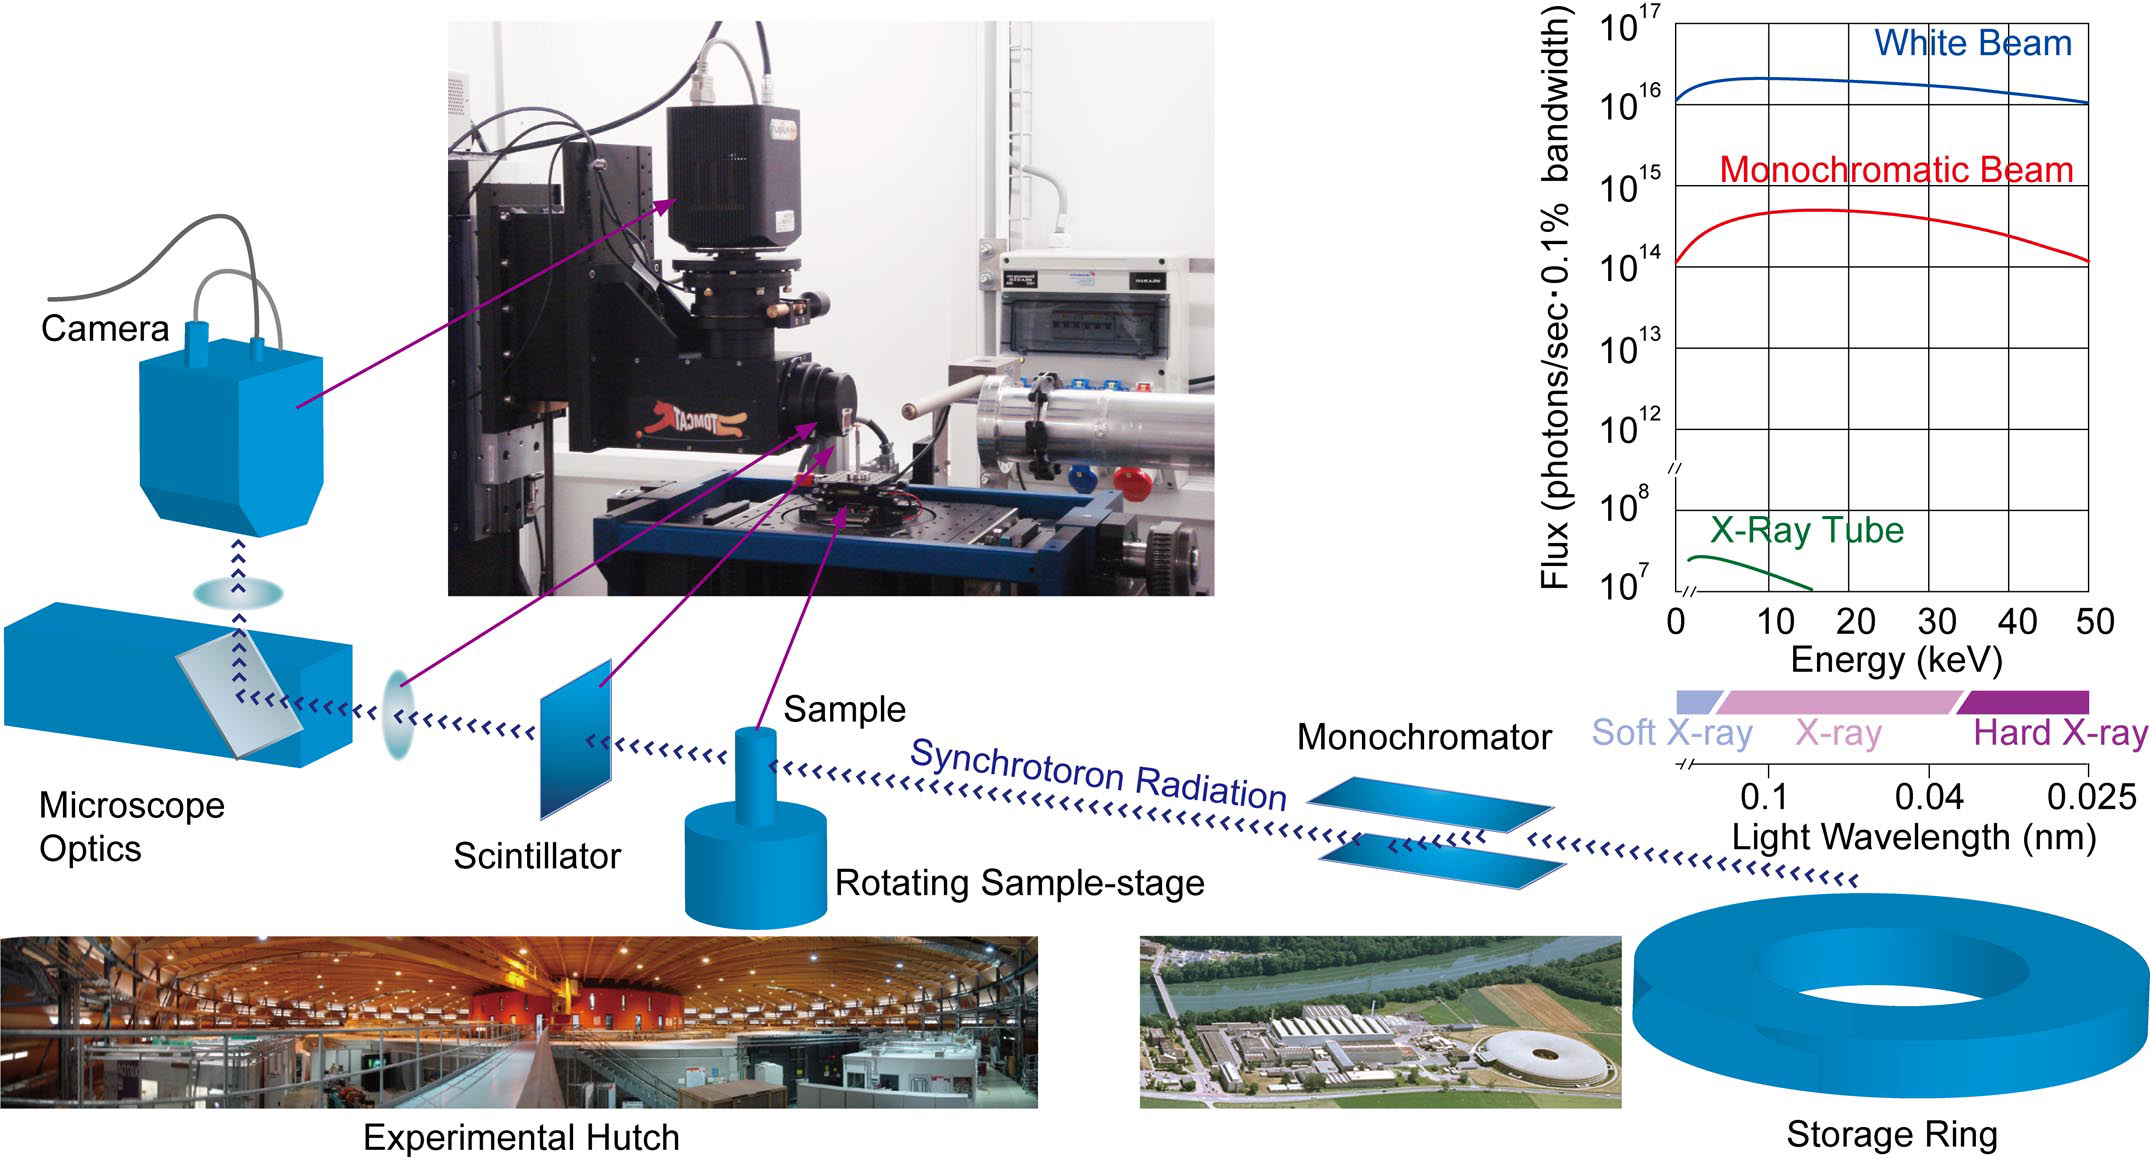
\includegraphics[width=\imsize]{img/Tsuda2008/Tsuda-02}%
	}%
	\caption[SRXTM imaging setup]{Imaging setup. The X-rays are coupled out of the storage ring via a wiggler. The monochromator is then used to select a desired wavelength of the incident X-rays. The sample is placed on a rotating sample holder inside the beam. While the X-rays penetrate the sample, the stage is rotated, and in total 1500 projections over \SI{180}{\degree} are recorded. Plot shows spectrum of \ac{tomcat} (red and blue) compared with conventional X-ray tube (green).}%
	\label{fig:imaging setup}%
\end{figure}

\subsubsection{Image manipulation}
To facilitate detailed analysis for the development of \threed acinar reconstruction image processing, a cubic subregion of varying size was selected from the full dataset using the software Imaris (Bitplane, Zürich, Switzerland) installed on an Athlon 64 3500 based personal computer. Different subregions were chosen, typically representing a particular tissue structure, such as a cluster of alveoli without any large airways/branches, as well as a region without prominent ring artifacts. Ring artifacts represent an intrinsic problem of tomographic images and in our case are caused by very small particles trapped on the scintillator. They are usually limited to only some sections of the stack of images and are more prominent in the center of the sample. Before proceeding with the next step, we reduced the noise in some of the original \twod images and softened the image edges by using a Gaussian filter and/or a median filter with a 1$\times$3$\times$3 kernel.

\subsubsection{Segmentation: thresholding and binarization}
To render our samples in three dimensions, we first segmented the raw data. Segmentation is the process of classifying the voxels of an image. Each voxel must represent either air space or tissue, thus, all the different gray values of the individual voxels are binarized into either 0 (air space) or 1 (lung tissue). Guided by the histogram of the gray scale values of the raw image (not shown), we selected an initial, tentative threshold value. Because the final selection of the threshold level is one of the most crucial steps in segmentation, special care has been taken to determine a correct threshold.

As indicated in \autoref{fig:workflow}, we determined the appropriate threshold level iteratively: 
\begin{enumerate}
	\item we set an initial threshold level and performed segmentation;
	\item we sequentially performed the object-connectivity analysis and \threed reconstruction of objects (described below);
	\item we calculated and compared morphological parameters, such as volume density of tissue and surface area density of air space to those given by \citet{Tschanz2003}; and
	\item we readjusted/reset the threshold level based on the results of \textit{step 3} if necessary.
\end{enumerate}

We performed this iterative process until the calculated morphological parameters closely matched the values of the gold standard~\cite{Tschanz2003}.

\subsubsection{Object connectivity analysis}
Depending on the threshold level selected, erroneous holes and isolated small areas/objects may appear in the segmented images. To avoid these artifacts and to maintain object connectivity, we needed to preprocess the segmented voxels. We first determined the number of isolated objects and their sizes in the \ac{roi} and then eliminated the objects below a reasonable size ($\sim$5 pixels) by reclassifying voxel values (from ``airway'' to ``tissue'', or vice versa). This \ac{oca} was performed by implementing label adjacent pixel analysis in \threed \cite{Ballard1982,Davies1990,Gonzalez1992}. For the sake of simplicity and clarity, we will explain this algorithm in \twod as follows.

\def\scale{0.5}
\begin{figure}
	\centering
	\noindent\makebox[\textwidth]{%
		\subfloat[]{%
			% !TEX root = ../Thesis.tex
%\documentclass{article}
%\usepackage{tikz}
%\usepackage[graphics,tightpage,active]{preview}
%\PreviewEnvironment{tikzpicture}
%\begin{document}
%\def\scale{1}
%%%%%%%%%%%%%%%%%%%%%%%%%%%%%%%%%%%%%%%%%%%%%%%%%%%%%%%%%%%%%%
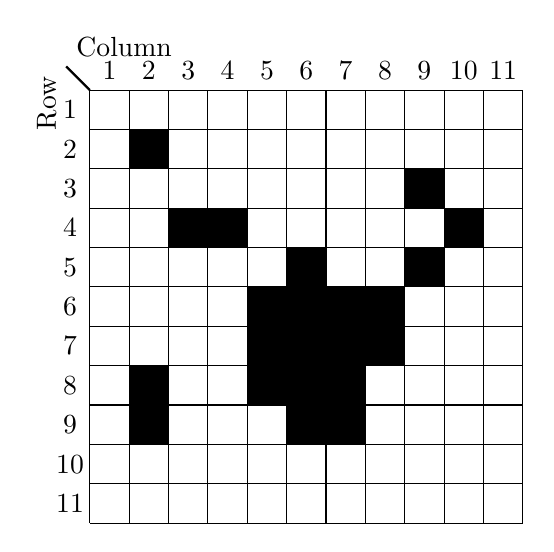
\begin{tikzpicture}[%
	scale=\scale,%
	number/.style ={white, text width=4em, text centered},%
	]
%%% grid
	\draw [thick] (0,0) -- (-.6,.6) node [anchor= south west] {Column} node [rotate=90,anchor= south east] {Row};
	\foreach \x in {0,...,11}
		{\draw (\x,0) -- (\x,-11);}
	\foreach \y in {0,...,-11}
		{\draw (0,\y) -- (11,\y);}
	\foreach \x in {1,...,11}
		\foreach \y in {0.5}
			{\draw (\x-.5,\y) node{\x};}
	\foreach \y/\label in {0/1,-1/2,-2/3,-3/4,-4/5,-5/6,-6/7,-7/8,-8/9,-9/10,-10/11}
		{\draw (-.5,\y-.5) node{\label};}
%%% grid
%%% fill
	\fill (1,-1) rectangle (2,-2);
	\fill (8,-2) rectangle (9,-3);
	\fill (2,-3) rectangle (4,-4);
	\fill (9,-3) rectangle (10,-4);
	\fill (5,-4) rectangle (6,-5);
	\fill (8,-4) rectangle (9,-5);
	\fill (4,-5) rectangle (8,-7);
	\fill (1,-7) rectangle (2,-9);
	\fill (4,-7) rectangle (7,-8);
	\fill (5,-8) rectangle (7,-9);
	%\fill (2,-9) rectangle (3,-10);
%%% fill
%%%% numbers
%	\node [number] at (1.5,-1.5) {1};
%	%
%	\node [number] at (8.5,-2.5) {2};
%	\node [number] at (9.5,-3.5) {2};
%	\node [number] at (9.5,-3.5) {2};
%	\node [number] at (8.5,-4.5) {\small 2/4};
%	%
%	\foreach \x in {2.5,3.5}
%		{\node [number] at (\x,-3.5) {3};}
%	%
%	\node [number] at (5.5,-4.5) {4};
%	\foreach \x in {4.5,...,6.5}
%	\foreach \y in {5.5,...,7.5}
%			{\node [number] at (\x,-\y) {4};}
%	\node [number] at (7.5,-5.5) {\small 4/2};
%	\node [number] at (7.5,-6.5) {4};
%	\foreach \x in {5.5,6.5}
%		{\node [number] at (\x,-8.5) {4};}
%	%
%	\foreach \y in {7.5,8.5}
%		{\node [number] at (1.5,-\y) {5};}
%	\node [number] at (2.5,-9.5) {5};
%%%% numbers
\end{tikzpicture}
%%%%%%%%%%%%%%%%%%%%%%%%%%%%%%%%%%%%%%%%%%%%%%%%%%%%%%%%%%%%%%
%\end{document}%
			\label{subfig:tsuda-03a}%
		}%
		\subfloat[]{%
			% !TEX root = ../Thesis.tex
%\documentclass{article}
%\usepackage{tikz}
%\usepackage[graphics,tightpage,active]{preview}
%\PreviewEnvironment{tikzpicture}
%\begin{document}
%\def\scale{1}
%%%%%%%%%%%%%%%%%%%%%%%%%%%%%%%%%%%%%%%%%%%%%%%%%%%%%%%%%%%%%%
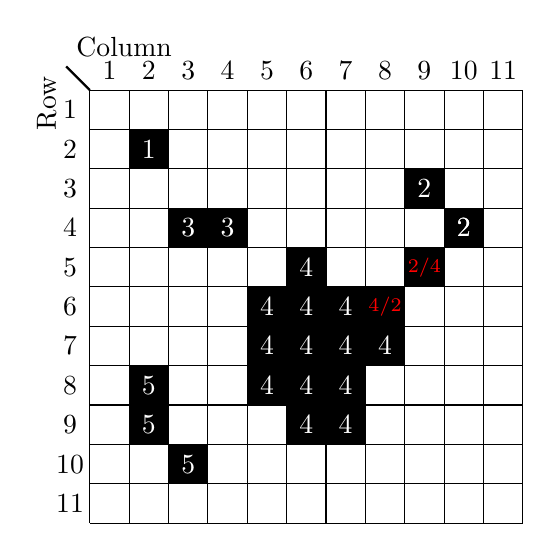
\begin{tikzpicture}[%
	scale=\scale,%
	number/.style ={white, text width=4em, text centered},%
	]
%%% grid
	\draw [thick] (0,0) -- (-.6,.6) node [anchor= south west] {Column} node [rotate=90,anchor= south east] {Row};
	\foreach \x in {0,...,11}
		{\draw (\x,0) -- (\x,-11);}
	\foreach \y in {0,...,-11}
		{\draw (0,\y) -- (11,\y);}
	\foreach \x in {1,...,11}
		\foreach \y in {0.5}
			{\draw (\x-.5,\y) node{\x};}
	\foreach \y/\label in {0/1,-1/2,-2/3,-3/4,-4/5,-5/6,-6/7,-7/8,-8/9,-9/10,-10/11}
		{\draw (-.5,\y-.5) node{\label};}
%%% grid
%%% fill
	\fill (1,-1) rectangle (2,-2);
	\fill (8,-2) rectangle (9,-3);
	\fill (2,-3) rectangle (4,-4);
	\fill (9,-3) rectangle (10,-4);
	\fill (5,-4) rectangle (6,-5);
	\fill (8,-4) rectangle (9,-5);
	\fill (4,-5) rectangle (8,-7);
	\fill (1,-7) rectangle (2,-9);
	\fill (4,-7) rectangle (7,-8);
	\fill (5,-8) rectangle (7,-9);
	\fill (2,-9) rectangle (3,-10);
%%% fill
%%%% numbers
	\node [number] at (1.5,-1.5) {1};
	%
	\node [number] at (8.5,-2.5) {2};
	\node [number] at (9.5,-3.5) {2};
	\node [number] at (9.5,-3.5) {2};
	\node [number,color=red] at (8.5,-4.5) {\scriptsize 2/4};
	%
	\foreach \x in {2.5,3.5}
		{\node [number] at (\x,-3.5) {3};}
	%
	\node [number] at (5.5,-4.5) {4};
	\foreach \x in {4.5,...,6.5}
	\foreach \y in {5.5,...,7.5}
			{\node [number] at (\x,-\y) {4};}
	\node [number,color=red] at (7.5,-5.5) {\scriptsize 4/2};
	\node [number] at (7.5,-6.5) {4};
	\foreach \x in {5.5,6.5}
		{\node [number] at (\x,-8.5) {4};}
	%
	\foreach \y in {7.5,8.5}
		{\node [number] at (1.5,-\y) {5};}
	\node [number] at (2.5,-9.5) {5};
%%%% numbers
\end{tikzpicture}
%%%%%%%%%%%%%%%%%%%%%%%%%%%%%%%%%%%%%%%%%%%%%%%%%%%%%%%%%%%%%%
%\end{document}%
			\label{subfig:tsuda-03b}%
		}%
	}\\% end makebox
	\noindent\makebox[\textwidth]{%
		\subfloat[]{%
			% !TEX root = ../Thesis.tex
%\documentclass{article}
%\usepackage{tikz}
%\usepackage[graphics,tightpage,active]{preview}
%\PreviewEnvironment{tikzpicture}
%\begin{document}
%\def\scale{1}
%%%%%%%%%%%%%%%%%%%%%%%%%%%%%%%%%%%%%%%%%%%%%%%%%%%%%%%%%%%%%%
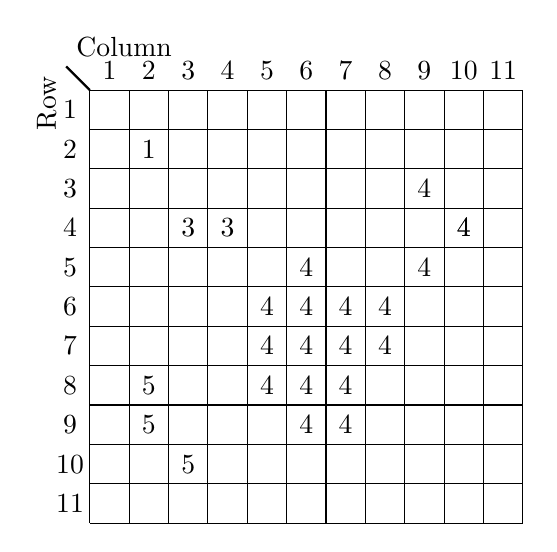
\begin{tikzpicture}[%
	scale=\scale,%
	number/.style ={black, text width=4em, text centered},%
	]
%%% grid
	\draw [thick] (0,0) -- (-.6,.6) node [anchor= south west] {Column} node [rotate=90,anchor= south east] {Row};
	\foreach \x in {0,...,11}
		{\draw (\x,0) -- (\x,-11);}
	\foreach \y in {0,...,-11}
		{\draw (0,\y) -- (11,\y);}
	\foreach \x in {1,...,11}
		\foreach \y in {0.5}
			{\draw (\x-.5,\y) node{\x};}
	\foreach \y/\label in {0/1,-1/2,-2/3,-3/4,-4/5,-5/6,-6/7,-7/8,-8/9,-9/10,-10/11}
		{\draw (-.5,\y-.5) node{\label};}
%%% grid
%%% fill
%	\fill (1,-1) rectangle (2,-2);
%	\fill (8,-2) rectangle (9,-3);
%	\fill (2,-3) rectangle (4,-4);
%	\fill (9,-3) rectangle (10,-4);
%	\fill (5,-4) rectangle (6,-5);
%	\fill (8,-4) rectangle (9,-5);
%	\fill (4,-5) rectangle (8,-7);
%	\fill (1,-7) rectangle (2,-9);
%	\fill (4,-7) rectangle (7,-8);
%	\fill (5,-8) rectangle (7,-9);
%	\fill (2,-9) rectangle (3,-10);
%%% fill
%%%% numbers
	\node [number] at (1.5,-1.5) {1};
	%
	\node [number] at (8.5,-2.5) {4};
	\node [number] at (9.5,-3.5) {4};
	\node [number] at (9.5,-3.5) {4};
	\node [number] at (8.5,-4.5) {4};
	%
	\foreach \x in {2.5,3.5}
		{\node [number] at (\x,-3.5) {3};}
	%
	\node [number] at (5.5,-4.5) {4};
	\foreach \x in {4.5,...,6.5}
	\foreach \y in {5.5,...,7.5}
			{\node [number] at (\x,-\y) {4};}
	\node [number] at (7.5,-5.5) {4};
	\node [number] at (7.5,-6.5) {4};
	\foreach \x in {5.5,6.5}
		{\node [number] at (\x,-8.5) {4};}
	%
	\foreach \y in {7.5,8.5}
		{\node [number] at (1.5,-\y) {5};}
	\node [number] at (2.5,-9.5) {5};
%%%% numbers
\end{tikzpicture}
%%%%%%%%%%%%%%%%%%%%%%%%%%%%%%%%%%%%%%%%%%%%%%%%%%%%%%%%%%%%%%
%\end{document}%
			\label{subfig:tsuda-03c}%
		}%
		\subfloat[]{%
			% !TEX root = ../Thesis.tex
%\documentclass{article}
%\usepackage{tikz}
%\usepackage[graphics,tightpage,active]{preview}
%\PreviewEnvironment{tikzpicture}
%\begin{document}
%\def\scale{1}
%%%%%%%%%%%%%%%%%%%%%%%%%%%%%%%%%%%%%%%%%%%%%%%%%%%%%%%%%%%%%%
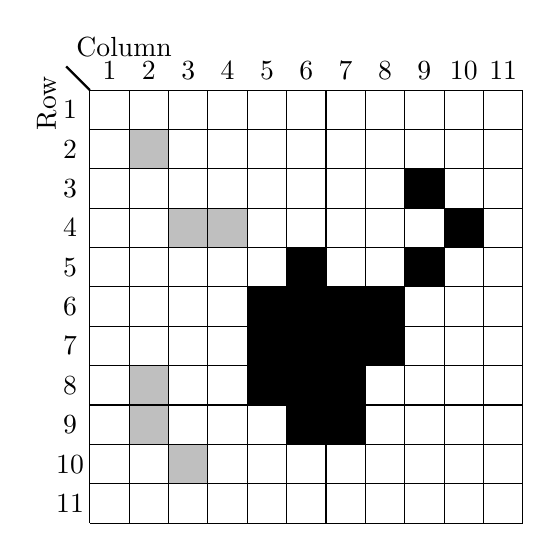
\begin{tikzpicture}[%
	scale=\scale,%
	number/.style ={white, text width=4em, text centered},%
	]
%%% fill
	\fill [fill=lightgray] (1,-1) rectangle (2,-2);
	\fill (8,-2) rectangle (9,-3);
	\fill [fill=lightgray] (2,-3) rectangle (4,-4);
	\fill (9,-3) rectangle (10,-4);
	\fill (5,-4) rectangle (6,-5);
	\fill (8,-4) rectangle (9,-5);
	\fill (4,-5) rectangle (8,-7);
	\fill [fill=lightgray] (1,-7) rectangle (2,-9);
	\fill (4,-7) rectangle (7,-8);
	\fill (5,-8) rectangle (7,-9);
	\fill [fill=lightgray] (2,-9) rectangle (3,-10);
%%% fill
%%% grid
	\draw [thick] (0,0) -- (-.6,.6) node [anchor= south west] {Column} node [rotate=90,anchor= south east] {Row};
	\foreach \x in {0,...,11}
		{\draw (\x,0) -- (\x,-11);}
	\foreach \y in {0,...,-11}
		{\draw (0,\y) -- (11,\y);}
	\foreach \x in {1,...,11}
		\foreach \y in {0.5}
			{\draw (\x-.5,\y) node{\x};}
	\foreach \y/\label in {0/1,-1/2,-2/3,-3/4,-4/5,-5/6,-6/7,-7/8,-8/9,-9/10,-10/11}
		{\draw (-.5,\y-.5) node{\label};}
%%% grid
%%%% numbers
%	\node [number] at (1.5,-1.5) {1};
%	%
%	\node [number] at (8.5,-2.5) {2};
%	\node [number] at (9.5,-3.5) {2};
%	\node [number] at (9.5,-3.5) {2};
%	\node [number] at (8.5,-4.5) {\small 2/4};
%	%
%	\foreach \x in {2.5,3.5}
%		{\node [number] at (\x,-3.5) {3};}
%	%
%	\node [number] at (5.5,-4.5) {4};
%	\foreach \x in {4.5,...,6.5}
%	\foreach \y in {5.5,...,7.5}
%			{\node [number] at (\x,-\y) {4};}
%	\node [number] at (7.5,-5.5) {\small 4/2};
%	\node [number] at (7.5,-6.5) {4};
%	\foreach \x in {5.5,6.5}
%		{\node [number] at (\x,-8.5) {4};}
%	%
%	\foreach \y in {7.5,8.5}
%		{\node [number] at (1.5,-\y) {5};}
%	\node [number] at (2.5,-9.5) {5};
%%%% numbers
\end{tikzpicture}
%%%%%%%%%%%%%%%%%%%%%%%%%%%%%%%%%%%%%%%%%%%%%%%%%%%%%%%%%%%%%%
%\end{document}%
			\label{subfig:tsuda-03d}%
		}%
	}%
	\caption[Object connectivity analysis]{Object connectivity analysis shown in a 2-dimensional (\twod) example. \subref{subfig:tsuda-03a}: a binary distribution of ``black'' vs.\ ``white'' pixels at certain threshold level; \subref{subfig:tsuda-03b}: An object label number (\acs{oln}) is assigned for each black pixel on the basis of the color (black or white) of 4 adjacent pixels; \subref{subfig:tsuda-03c}: on the basis of a ``flag'' pixel (red text in panel \subref{subfig:tsuda-03b}), connectivity is identified between \ac{oln}=2 and \ac{oln}=4; \subref{subfig:tsuda-03d}: small objects less than cutoff (=4 pixels in this example, light gray) are removed.}
	\label{fig:tsuda-03}
\end{figure}

Let us assume that ``black'' and ``white'' pixels (voxels in a \threed case) are distributed as in the example shown in \autoref{subfig:tsuda-03a}. Scanning pixels from top to bottom and from left to right, we will examine the connectivity of each black pixel, by checking the colors (black or white) of its four adjacent pixels [a pixel on its left and three pixels on its top (top left, top middle, top right)]. We will assign a tentative \acf{oln} (consecutively, 1, 2, 3, 4\ldots) to each black pixel and examine connections between identified objects. Four simple logical algorithms are involved.
\begin{enumerate}
	\item If all four adjacent pixels are white, assign a new \ac{oln} to the current black pixel. [For instance, we assign \ac{oln}=1 to the pixel at (column 2; row 2); \ac{oln}=2 to the pixel at (9;3), etc. (\autoref{subfig:tsuda-03b}).]
	\item If only one of the adjacent pixels has already been assigned an \ac{oln}, assign the same \ac{oln} to the current black pixel. [For instance, we assign the \ac{oln}=3 to the pixel at (4;4) because the adjacent pixel on the left of it (at 3;4) has already been assigned with \ac{oln}=3 (\autoref{subfig:tsuda-03b}).]
	\item If more than one adjacent pixels have already been assigned an \ac{oln} and if those adjacent pixels have the same \ac{oln}, assign the same \ac{oln} to the current pixel. [For instance, we assign \ac{oln}=4 to the pixel at (6;6) because the adjacent pixels at (5;6) and at (6;5) have already been assigned with an \ac{oln}=4 (\autoref{subfig:tsuda-03b}).]
	\item If more than one adjacent pixel has already been assigned an \ac{oln} but if those adjacent pixels have different \acp{oln}, assign one of the adjacent pixel's \ac{oln} and put a special marker (flag) on that pixel. The pixel with this flag will be re-examined in the next step. [For instance, we assign either \ac{oln}=2 or 4 to the pixel at (8;6) because the adjacent pixels at (9;5) and at (7;6) have already been assigned with \ac{oln}=2 and 4, respectively. Thus, the pixel is marked with a flag (shown red in \autoref{subfig:tsuda-03b}).]
\end{enumerate}
After assigning \acp{oln} to all the black pixels, we then re-examine the flagged pixels, which indicate that two or more ``appeared-to-be separated'' objects are indeed connected. We reassign the same \ac{oln} to all of the connected pixels leaving from the flagged pixel. For instance, we assigned \ac{oln}=4 to the pixel at (8;6). This means that the pixels (9; 3), (10; 4) and (9; 5) are also assigned with the \ac{oln}=4 (\autoref{subfig:tsuda-03c}). Finally, we remove small objects that are physically unreasonable in size ($<$5 pixels; \autoref{subfig:tsuda-03d}), suppressing noise and artifacts from the image acquisition.

\subsubsection{\threed reconstruction of separated objects}
Much of the currently available medical imaging software for \threed reconstruction treats objects (\ie, lung tissues in our case) as surfaces, and this is most often done by a triangulation of the voxel surface. However, to perform a complete \threed reconstruction, we use a different approach here; we reconstruct not only the surface of the boundary between the tissue and the air space, but also the volumes of tissues and air space by fitting \ac{fe} to the raw voxel data and hence inside the full volume. For this, we use a \ac{gbha}~\cite{Schneiders1996}, which is explained as follows.

Let us consider an example in which we want to apply a threshold of 123 for the segmentation of our images. In \autoref{subfig:tsuda-04a}, at \textit{left} the thresholded voxels in a \threed representation is shown and, for the sake of discussion and clarity, a \twod representation is shown at \textit{right}.
\begin{description}
	\item[1. Mesh generation] A \ac{fe} mesh (\autoref{subfig:tsuda-04b}), initially uniform, is isotropically generated over all pixels. We position the nodes of the \ac{fe} mesh at the centers of the existing voxels (\autoref{subfig:tsuda-04b}, \textit{right}). This means that each \ac{fe} overlaps 2$\times$2 voxels in the \twod case. (\autoref{subfig:tsuda-04b}, \textit{right}) or 2$\times$2$\times$2 voxels in the \threed case (\autoref{subfig:tsuda-04b}, \textit{left}). The black circles represent nodes generated inside the object and the white circles denote nodes outside of the object. The nodes inside the object have a pixel or voxel value higher than the chosen threshold and the nodes outside the object have a value lower than the chosen threshold. Each \ac{fe} node is assigned the grayscale value of the corresponding voxel. Note that the boundary between the black and white nodes is not smooth at this stage.
	\item[2. Surface smoothing I] Because the \ac{fe} mesh is located on the surface boundary, some of its nodes (shown as the white circles) are on the outside of the object. Additionally, the grayscale pixel values of those white nodes are lower than the chosen threshold value. By using a simple linear interpolation, we move these white nodes in the direction of the surface boundary toward the locations where the grayscale pixel value would exactly match the threshold value. There are multiple methods available to move the nodes by linear interpolation. We adapted the method developed by \citet{Schneiders1996} for our \threed case. It is important to note that in some cases, this linear interpolation might even move the node inside the object (see \autoref{subfig:tsuda-04c} for examples).
	\item[3. Surface smoothing II] The translation of the nodes as described in \textit{step 2} may in some cases lead to a distorted (concave) \ac{fe} surface. The distortion of the \ac{fe} nodes can be evaluated with their Jacobian value. The Jacobian value is a matrix of the derivation of global to local \ac{fe} interpolation function and the quality of any mesh can be directly evaluated by its Jacobian value~\cite{Bathe1995}. Distorted \acp{fe}, which are not suitable for subsequent numerical calculations, show a negative Jacobian. To optimize the Jacobian, we implemented the standard \ac{lst}~\cite{Freitag2000}). The \ac{lst} usually takes a few loops (repetitions of \textit{step 2}) over all \acp{fe} to achieve positive Jacobian values for all \acp{fe}. The results of applying the \ac{lst} for \threed and \twod cases are shown, respectively, in \autoref{subfig:tsuda-04d}, \textit{right} (``After \ac{lst}'').
\end{description}

\renewcommand{\imsize}{.75\linewidth}
\begin{figure}
	\noindent\makebox[\textwidth]{%
		\subfloat[]{%
			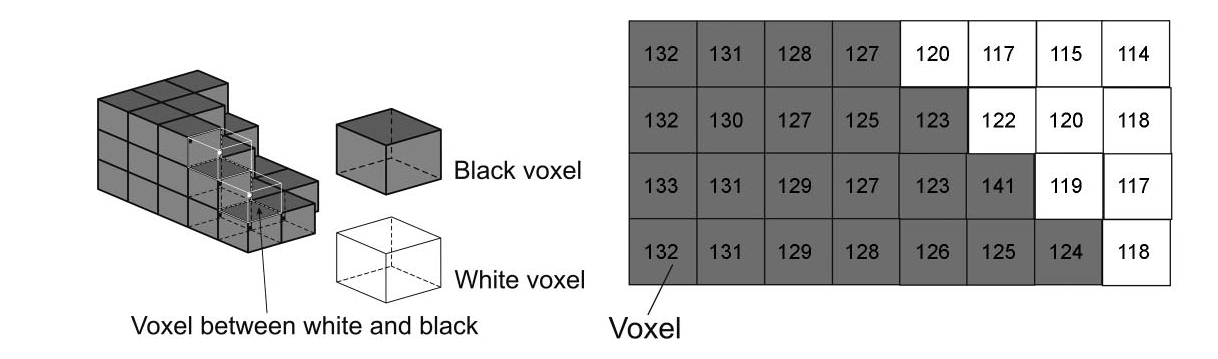
\includegraphics[width=\imsize]{img/Tsuda2008/Tsuda-04a}%
			\label{subfig:tsuda-04a}%
		}%
	}\\%
	\noindent\makebox[\textwidth]{%
		\subfloat[]{%
			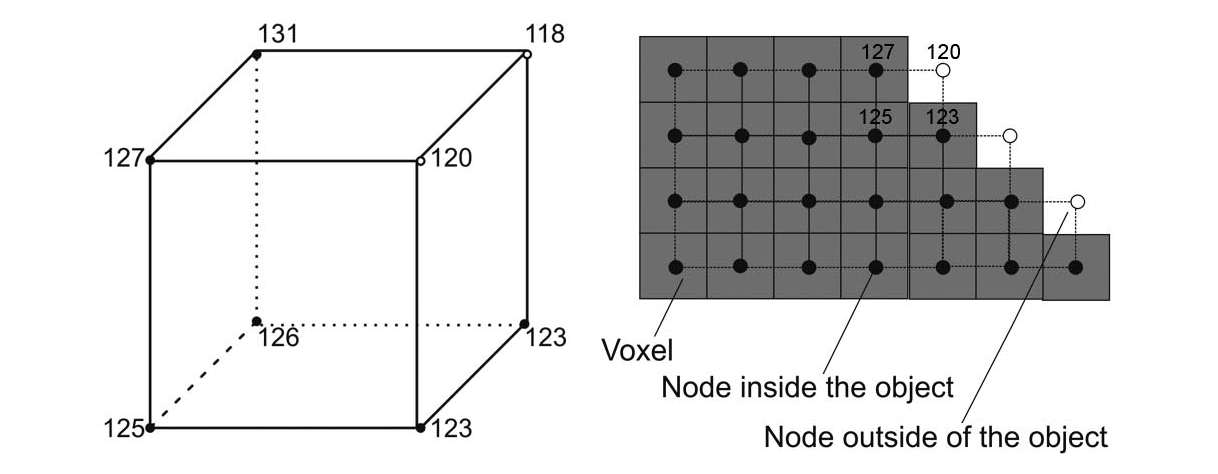
\includegraphics[width=\imsize]{img/Tsuda2008/Tsuda-04b}%
			\label{subfig:tsuda-04b}%
		}%
	}\\%
	\noindent\makebox[\textwidth]{%
		\subfloat[]{%
			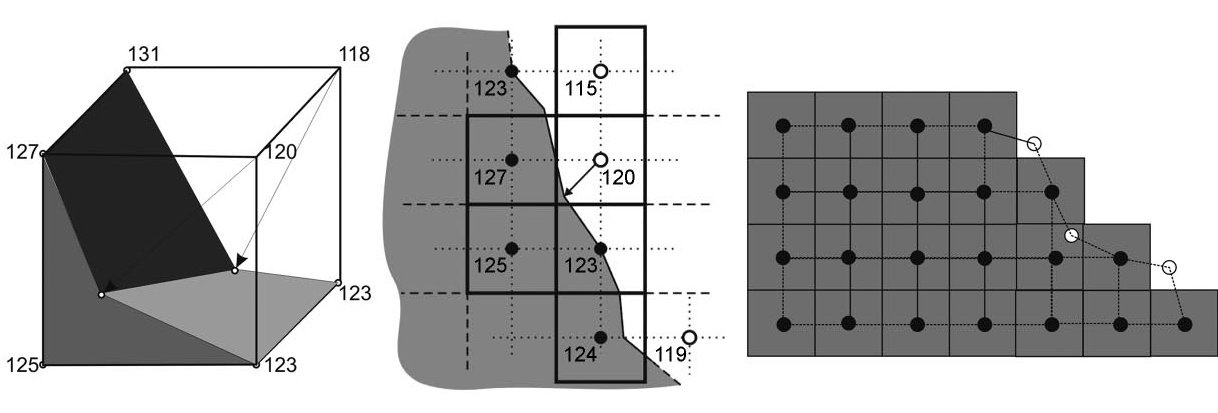
\includegraphics[width=\imsize]{img/Tsuda2008/Tsuda-04c}%
			\label{subfig:tsuda-04c}%
		}%
	}\\%
	\noindent\makebox[\textwidth]{%
		\subfloat[]{%
			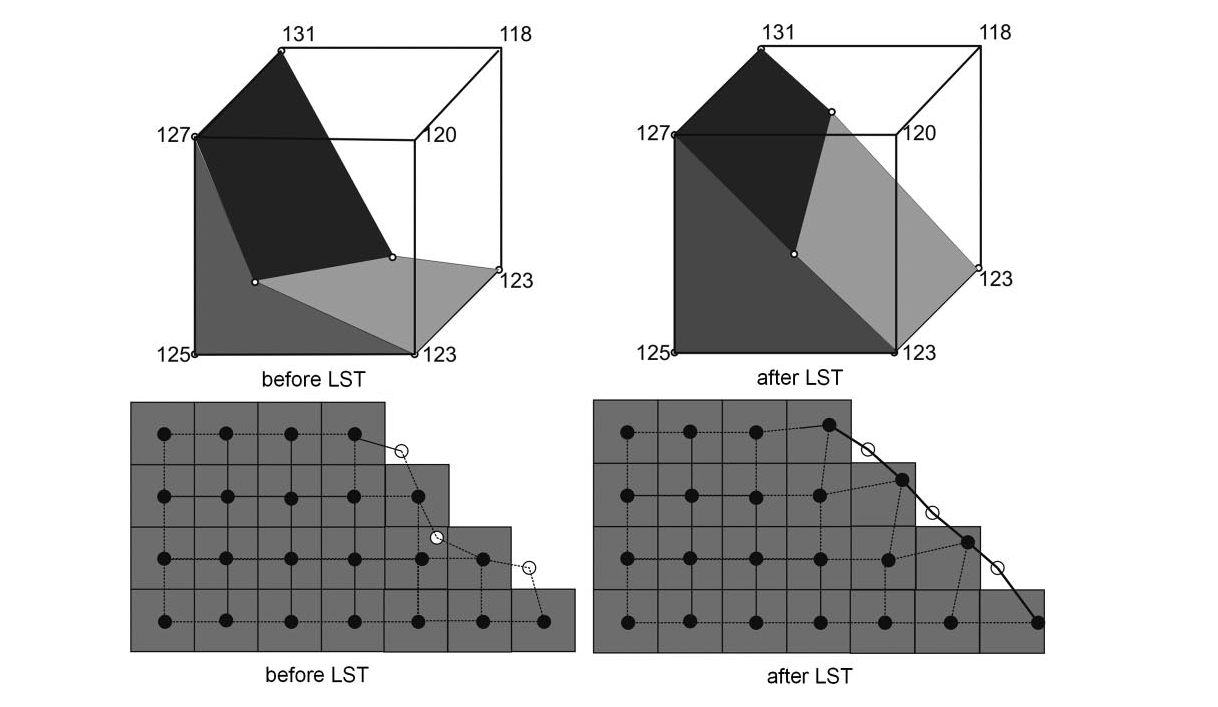
\includegraphics[width=\imsize]{img/Tsuda2008/Tsuda-04d}%
			\label{subfig:tsuda-04d}%
		}%
	}%
	\caption[Grid-based hexahedral algorithm]{Grid-based hexahedral algorithm. \subref{subfig:tsuda-04a}: \threed thresholded voxels (\textit{left}) and \twod representation of thresholded voxels (\textit{right}). The grayscale values are kept in the map of voxel. \subref{subfig:tsuda-04b}: step 1: generation of uniform \acl{fe} mesh over the voxel map. For simplicity, \ac{fe} nodes are positioned at the center of voxel. \threed \ac{fe} meshing (\textit{left}) and \twod \ac{fe} meshing (\textit{right}) are shown. Each node is assigned with the grayscale value from the corresponding voxel. \subref{subfig:tsuda-04c}: step 2: moving nodes on the surface due to trilinear interpolation in \threed case (\textit{left}) and bilinear interpolation in \twod case (\textit{right}). The location of surface boundary is shown in the middle image for \twod case. A fast sub \ac{fe}-voxel level algorithm is implemented to locate a surface boundary. White nodes are moving toward this surface boundary. \subref{subfig:tsuda-04d}: step 3: \acf{lst}. \threed and \twod before \ac{lst} (\textit{left}), \threed and \twod after \ac{lst} (\textit{right}).}
	\label{fig:tsuda-04}
\end{figure}

\subsection[Validation of Segmentation]{Validation of Segmentation and Image Processing}
Once \threed reconstruction was performed with a certain tentative threshold value, the resulting \threed structure was evaluated against the gold standard, \ie, well-characterized morphometric data provided by \citet{Tschanz2003}. We calculated the volume density of tissue (V\textsubscript{VS}) and surface area density of air space (S\textsubscript{VS}~[\centimetresquared\per\centimetrecubed]) to determine if there was unacceptable discrepancy. If so, we readjusted the threshold level and repeated the segmentation process, mesh generation, and subsequent image analysis until our calculated morphological parameters were within $<$\SI{5}{\percent} difference of the gold standard (\autoref{fig:workflow}).

\subsection[Visualization of the Reconstruction]{Visualization of the \threed Reconstruction}
Once the calculated morphological parameters met the gold standard, the resulting \threed reconstruction was transformed in a standard \acs{vrml} format for visualization as well as a proprietary DAT format for subsequent \ac{fe} analysis.

\section{Results}
The Epon embedded lung tissue samples of a 60-day-old rat were selected from the ``lung tissue library'' of Peter Burri's lab (University of Bern). All morphological parameters of this particular rat, against which our data were compared, are available and published in~\citet{Tschanz2003}.

\subsection{A Raw Image Stack and a Cubic Subregion}
The samples were scanned with \ac{srxtm} and a stack of 1024 raw images was reconstructed in tiff format (\autoref{subfig:tsuda-05a}: stack of images, \ref{subfig:tsuda-05b}: one slice of the raw data). The resolution of the image was \SI{1.4}{\micro\meter} per pixel, thus the edge length of the cubic stack was \SI{1.4336}{\milli\meter}, containing approximately one billion isotropic voxels.

To facilitate further processing of the image, different subregions of interest were extracted from the original raw data (one exemplary \ac{roi} is the orange small cube in \autoref{subfig:tsuda-05a}, which is shown enlarged in \autoref{subfig:tsuda-05c}. This \ac{roi} has a size of 196$\times$196$\times$196 pixels (\ie, an edge length of $\sim$\SI{275}{\micro\meter}) and contains $\sim$7.5 million voxels. This is a reasonable size of data that can easily be handled by a standard \acsu{pc} (Duo Core 2 Pentium \SI{2.33}{\gigahertz}, \SI{2}{\giga\byte} \acs{ram}) for visualization and volume rendering. The aforementioned size is an intermediate \ac{roi}; depending on the need for visualization/volume rendering other sizes have been chosen. To validate the segmentation (see below), we split a big \ac{roi} inside the sample in the full dataset vertically into five subregions leading to a \ac{roi} size of 200$\times$200$\times$180 pixels.

\renewcommand{\imsize}{0.705\linewidth}%
\begin{figure}
	\noindent\makebox[\textwidth]{%
		\subfloat[]{%
			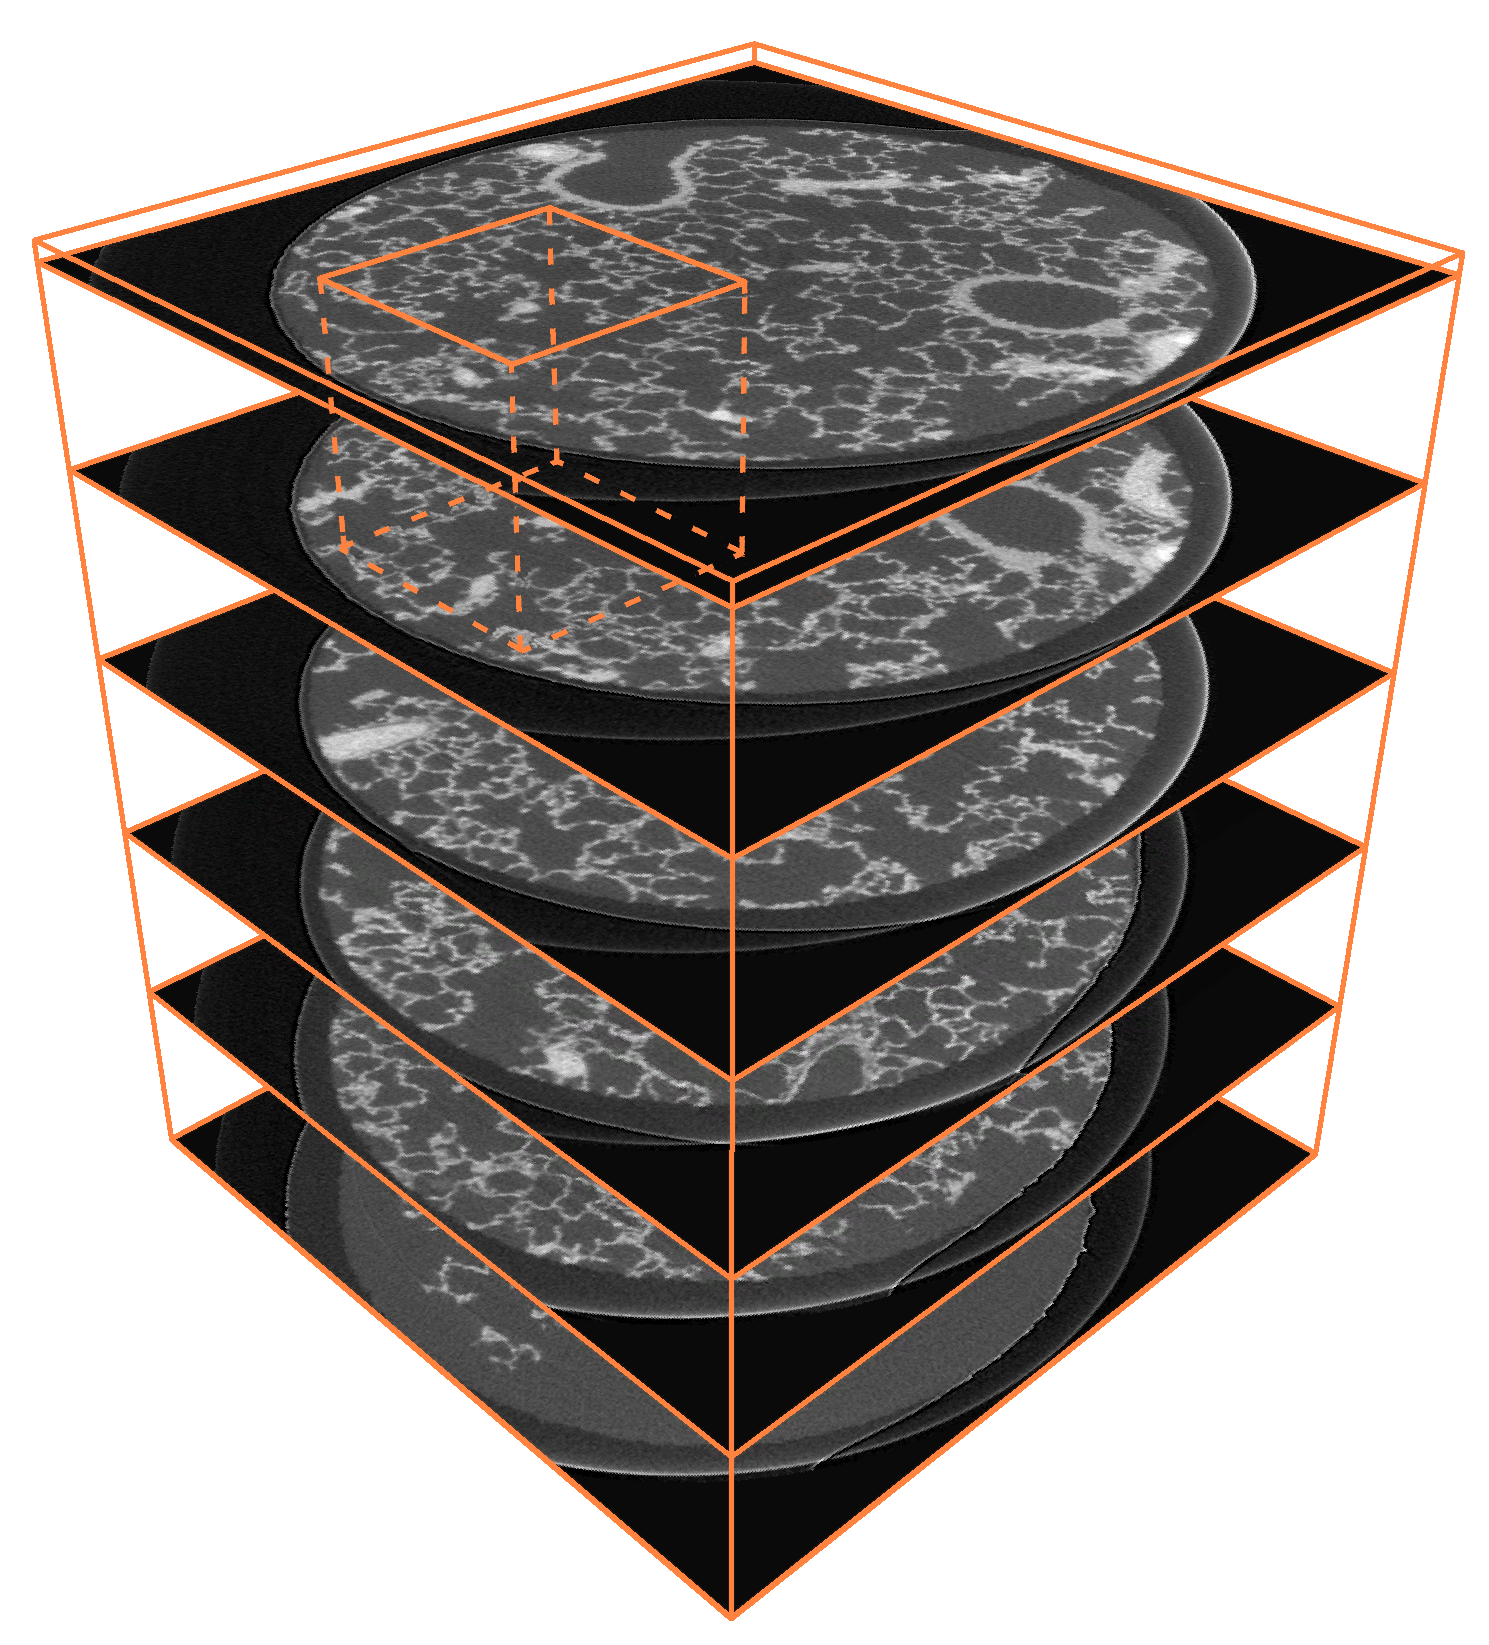
\includegraphics[width=\imsize]{img/Tsuda2008/Tsuda-05a}%
			\label{subfig:tsuda-05a}%
		}\hfill%
		\subfloat[]{%
			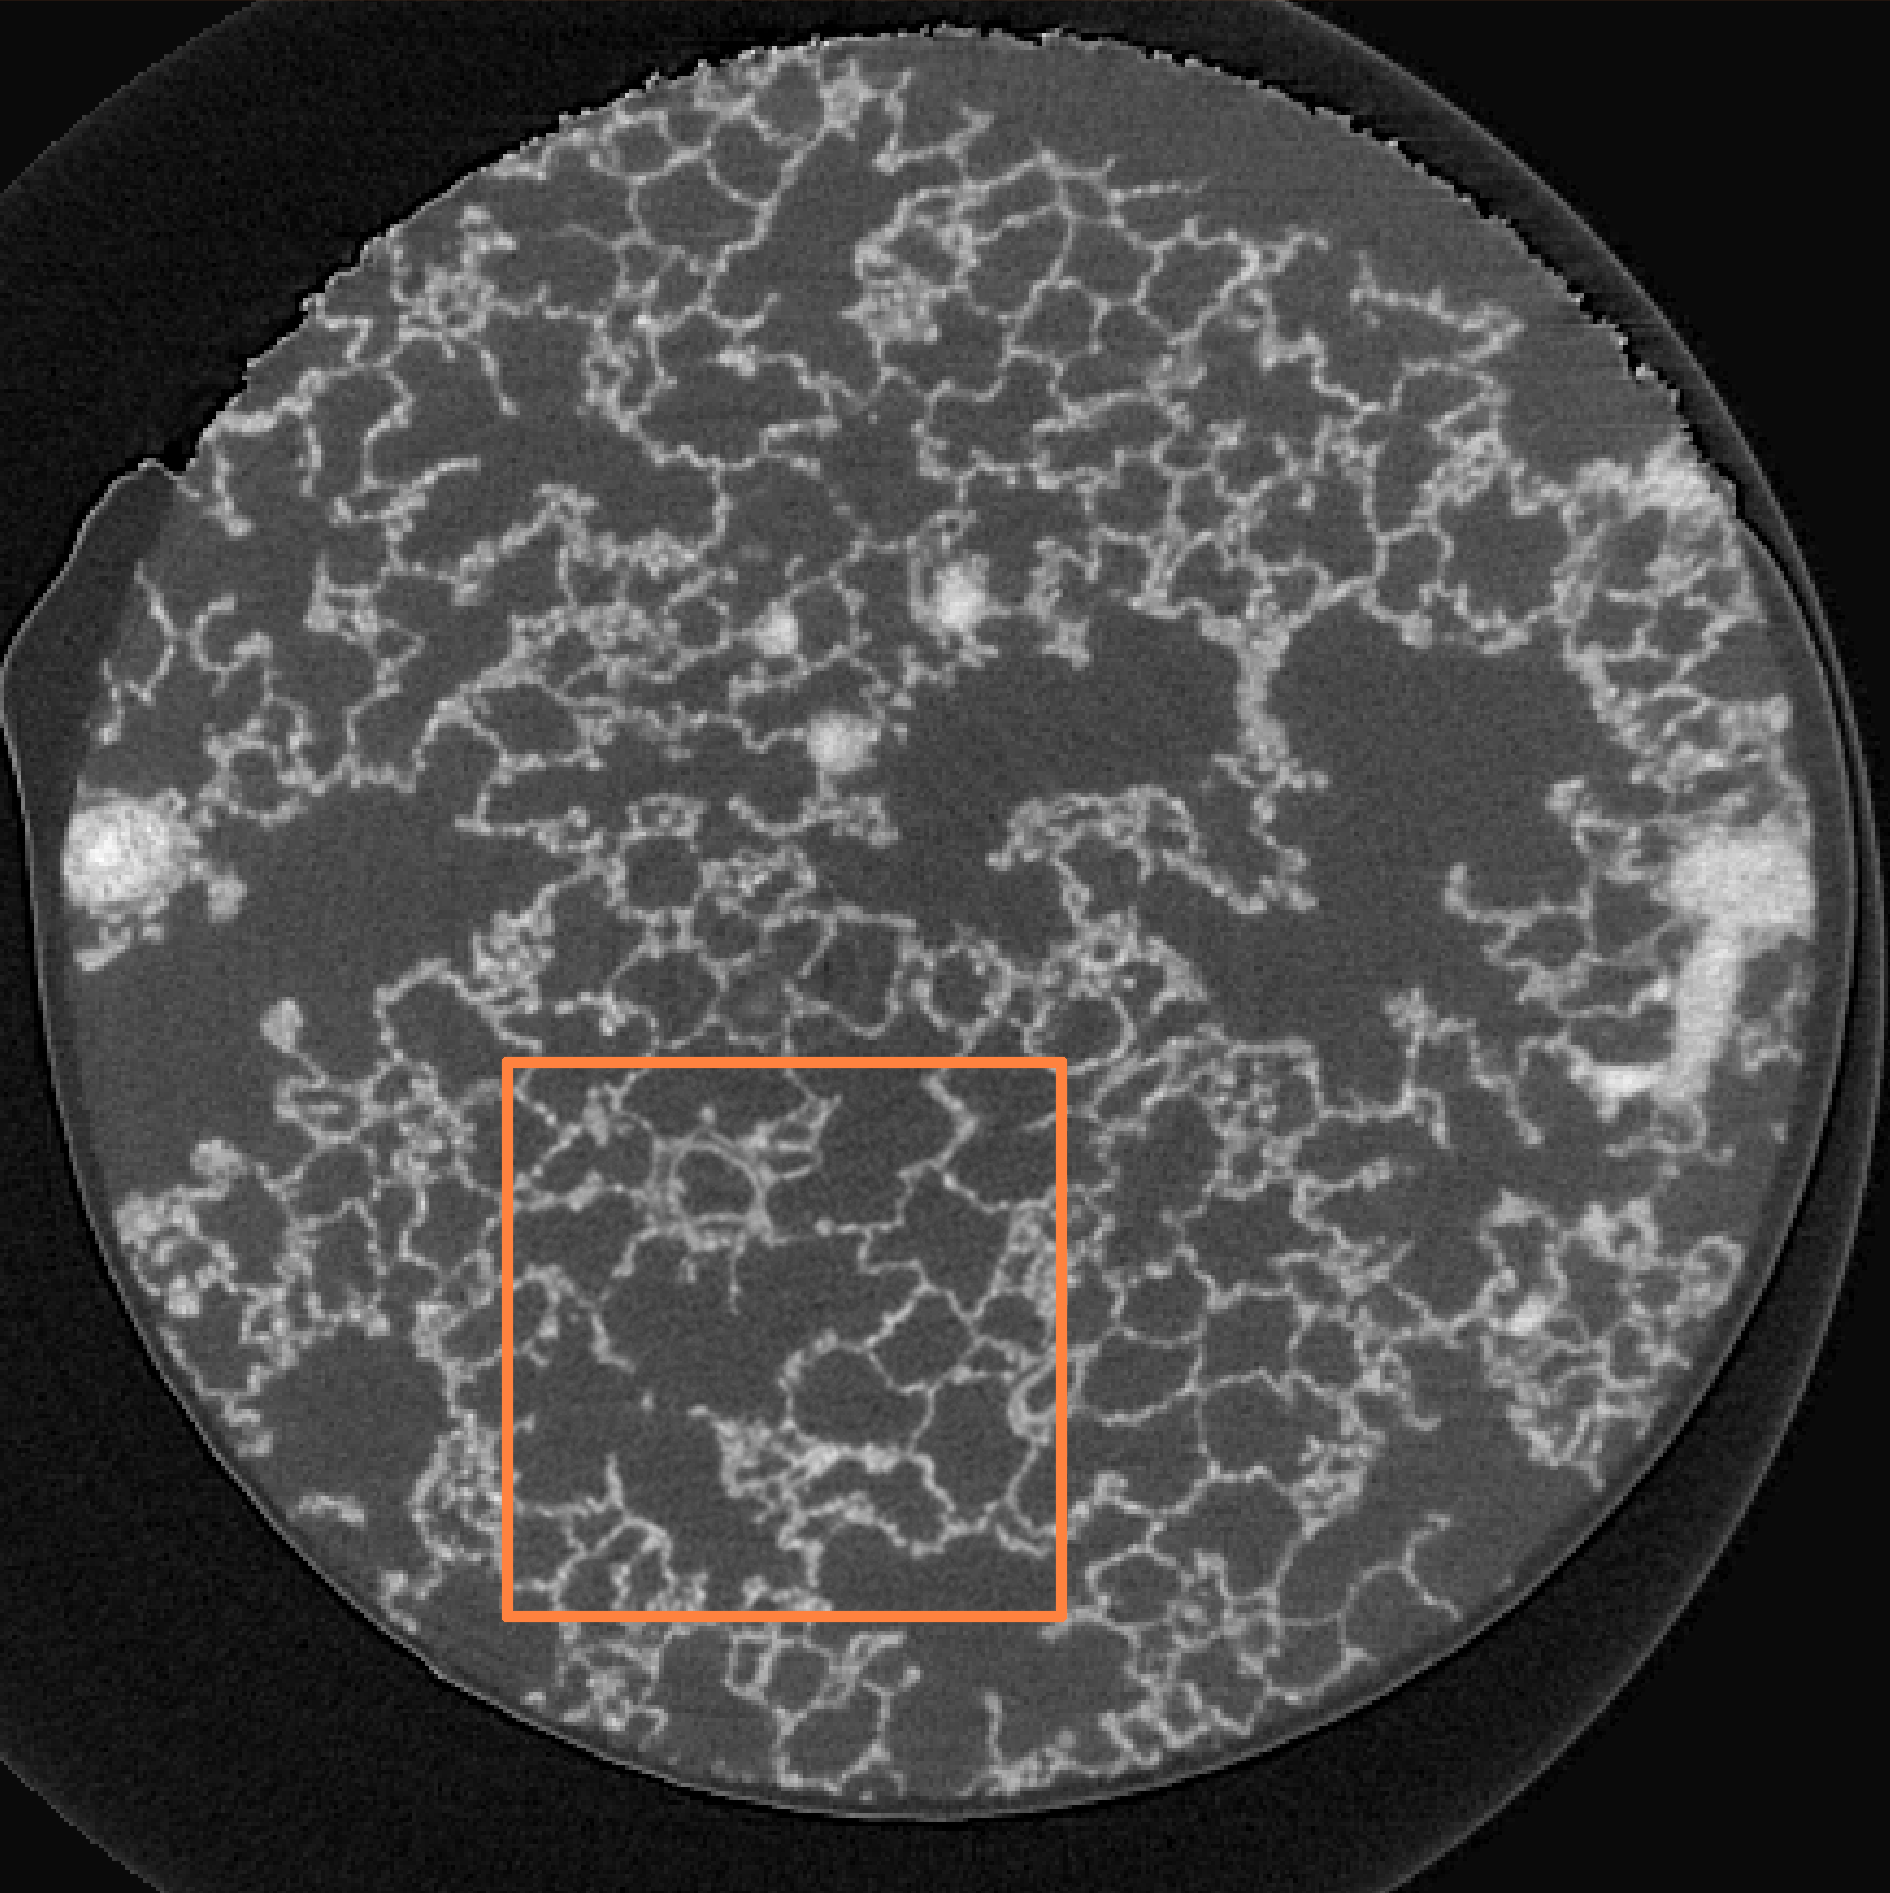
\includegraphics[width=\imsize]{img/Tsuda2008/Tsuda-05b}%
			\label{subfig:tsuda-05b}%
		}%
	}%
	\\%
	\noindent\makebox[\textwidth]{%
		\subfloat[]{%
			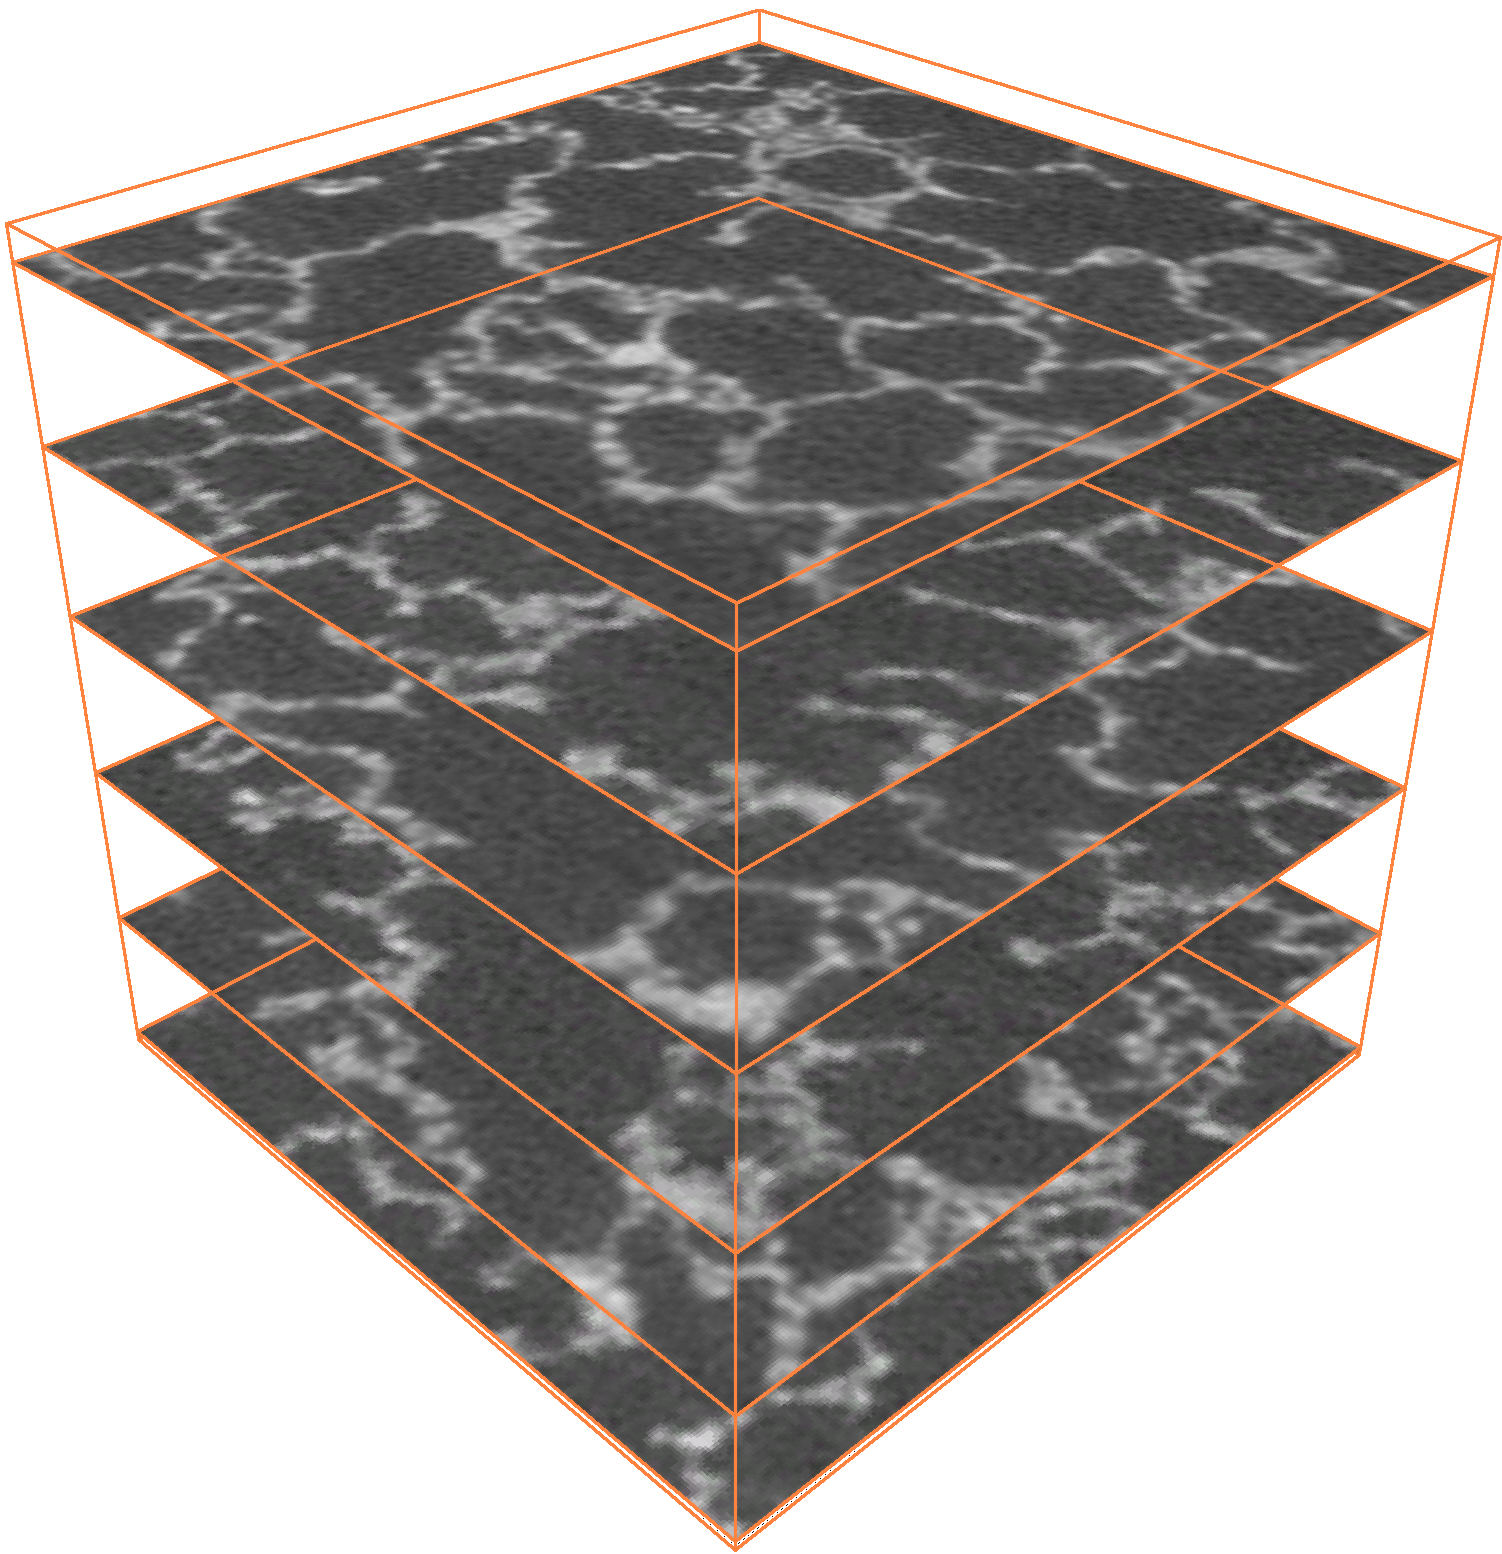
\includegraphics[width=\imsize]{img/Tsuda2008/Tsuda-05c}%
			\label{subfig:tsuda-05c}%
		}\hfill%
		\subfloat[]{%
			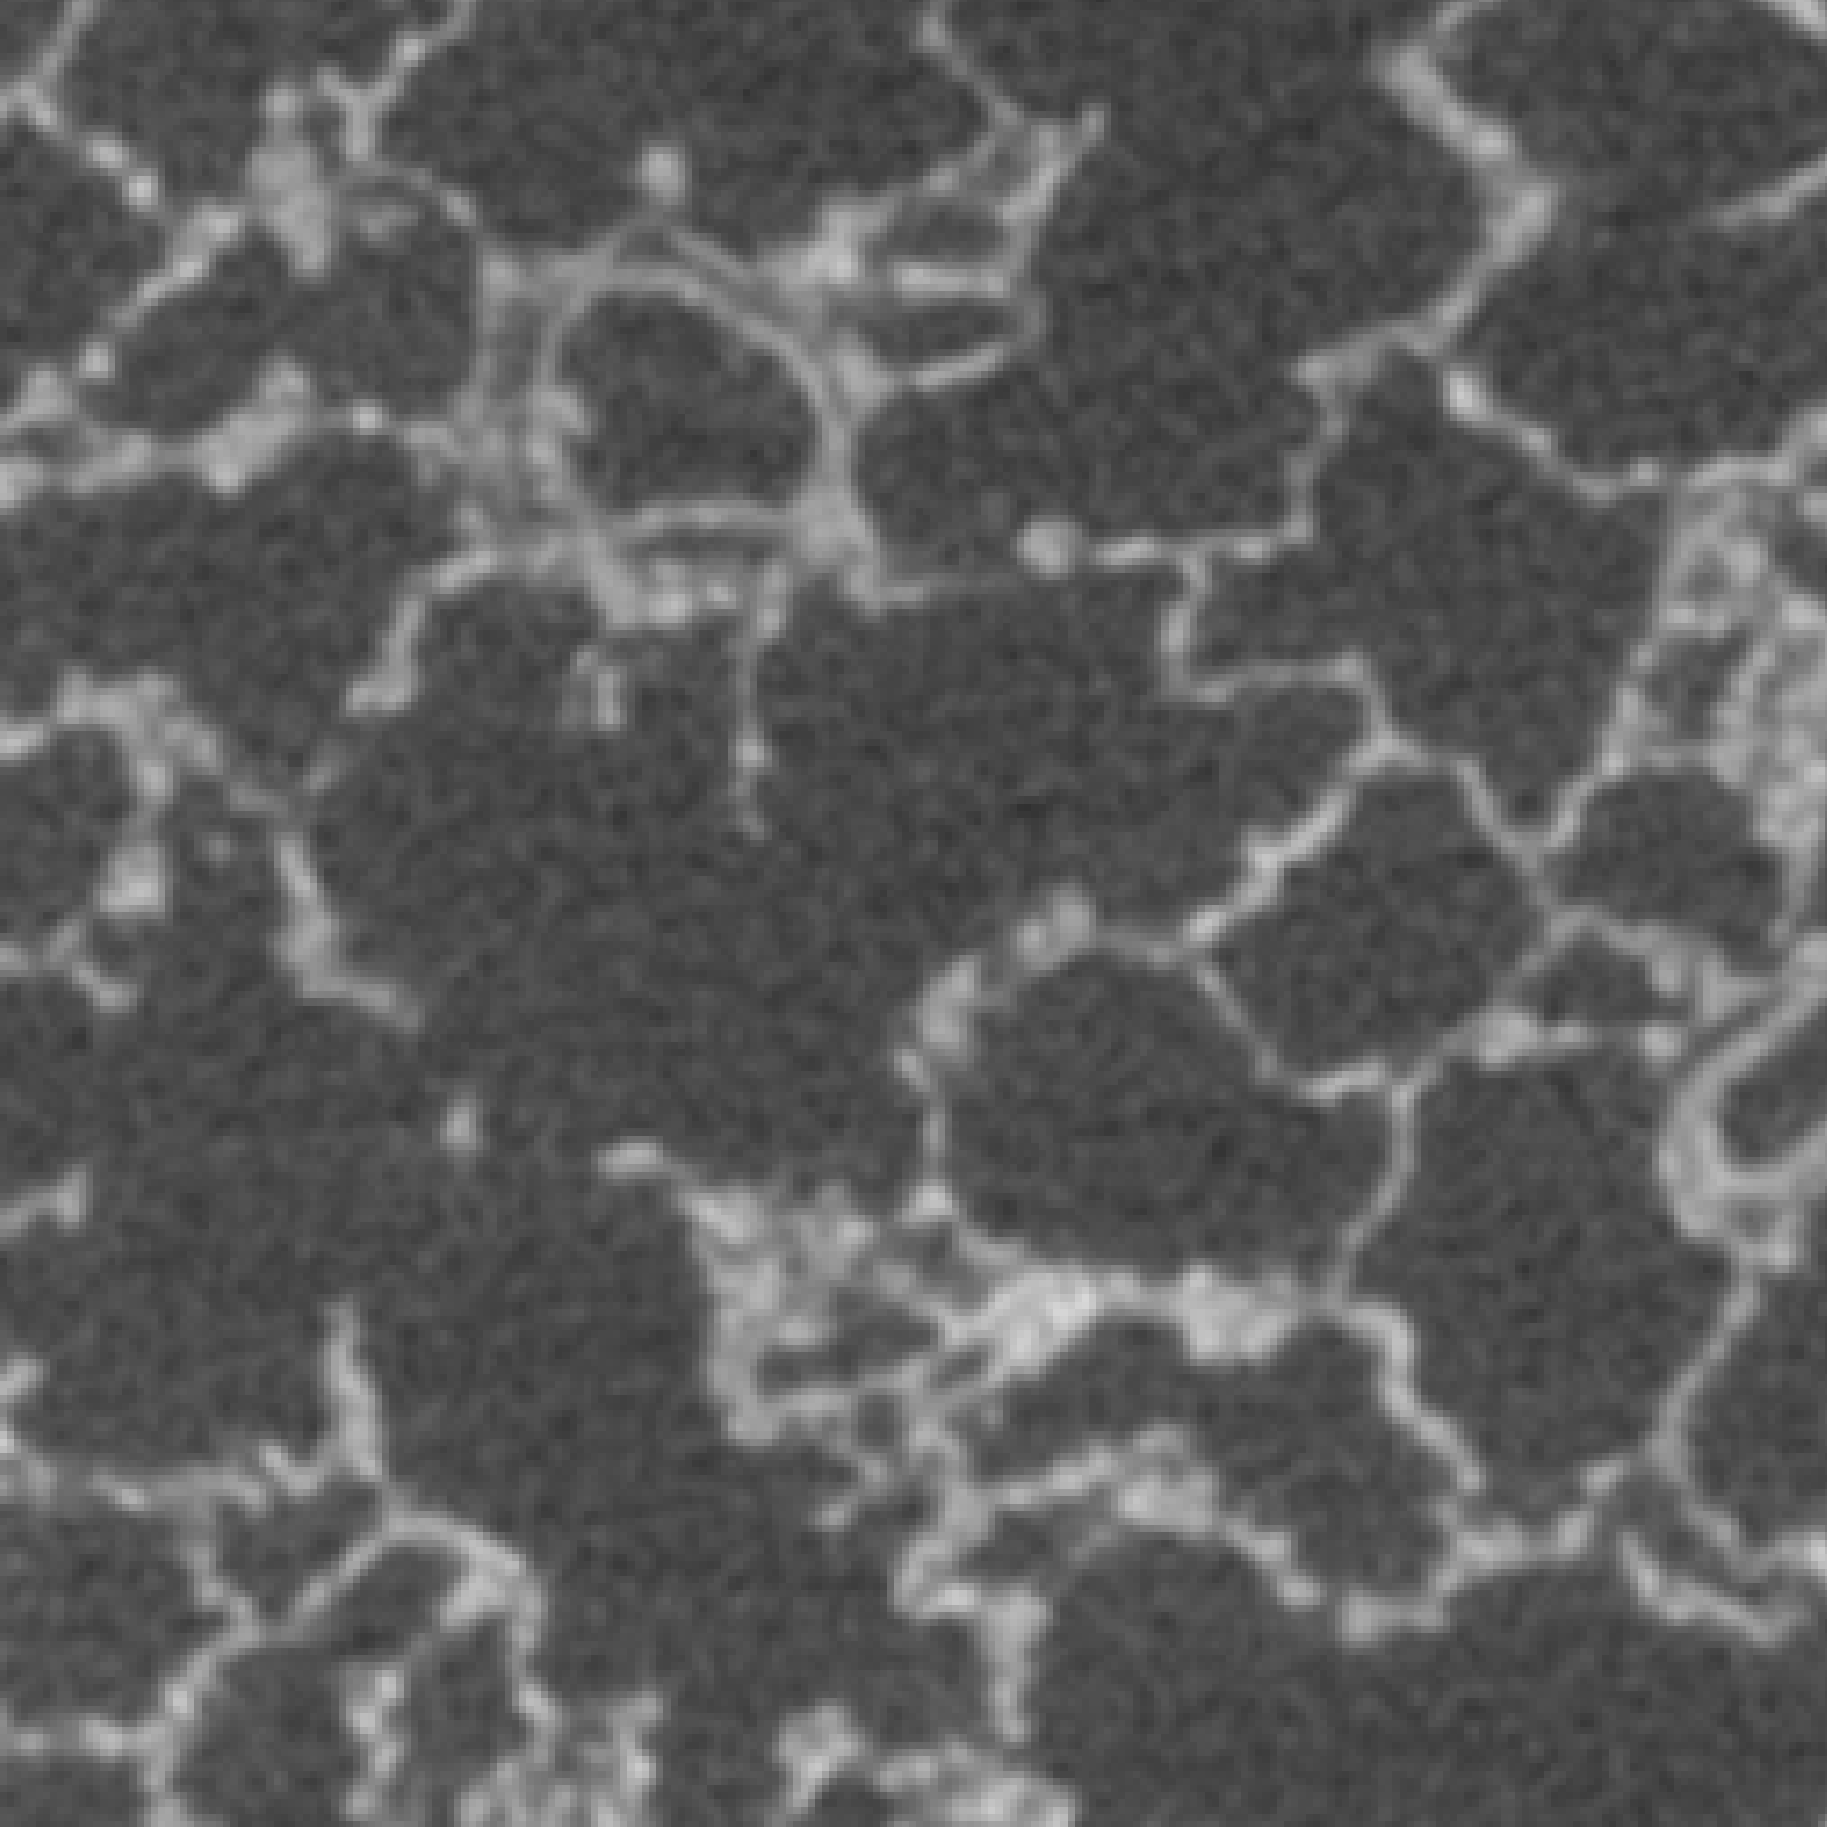
\includegraphics[width=\imsize]{img/Tsuda2008/Tsuda-05d}%
			\label{subfig:tsuda-05d}%
		}%
	}%
	\caption[Overview of workflow for the selection of a region of interest]{Overview of workflow for the selection of a \acf{roi}. \subref{subfig:tsuda-05a}: full perspective view of the sample R108C60C-07e with 6 selected orthogonal slices and bounding box of the full sample in orange. The \ac{roi} selected for subfigures \subref{subfig:tsuda-05c} and \subref{subfig:tsuda-05d} is visible in the \textit{top left}. \subref{subfig:tsuda-05b}: close-up of one slice of the full dataset with selected \ac{roi} (side-length of 256 pixels). \subref{subfig:tsuda-05c}: \ac{roi} cut out of the full sample, 6 selected orthogonal slices are shown. \subref{subfig:tsuda-05d}: close-up of the \ac{roi} in subfigure \subref{subfig:tsuda-05b}.}
	\label{fig:tsuda-05}
\end{figure}

\subsection{Segmentation}
As mentioned, the selection of a threshold level has significant affects on segmentation. To demonstrate this, we have segmented a small crop of the original data (\autoref{subfig:tsuda-06a}) with three different threshold values. With a low threshold level, for instance 130, the image would possess too many black voxels and the septa in the lung appear to be too thick (\autoref{subfig:tsuda-06b}). On the other hand, with a higher threshold level, for instance 148, the image would possess too many white voxels and the lung tissue appears to be very thin, with multiple erroneous holes in the septal walls (\autoref{subfig:tsuda-06d}). With an intermediate threshold, for instance 139, the lung structure appears to be reasonable, with a minor amount of holes (\autoref{subfig:tsuda-06c}). The optimal value of the threshold level was iteratively determined by performing a ``readjustment-recalculation'' process to match some of the key morphological parameters in the resulting \threed reconstruction to the gold standard. This is explained below in detail.

\renewcommand{\imsize}{0.47\linewidth}
\setlength{\fboxsep}{-\fboxrule}
\begin{figure}
	\noindent\makebox[\textwidth]{%
		\subfloat[]{%
			\pgfmathsetlength{\imagewidth}{\imsize}%
			\pgfmathsetlength{\imagescale}{\imagewidth/238}%
			\begin{tikzpicture}[x=\imagescale,y=-\imagescale]
				\def\x{127} % scalebar-x at golden ratio of x=238px
				\def\y{214} % scalebar-y at 90% of height of y=238px
				\node[anchor=north west, inner sep=0pt, outer sep=0pt] at (0,0) {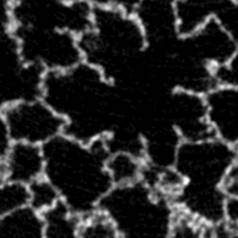
\includegraphics[width=\imagewidth]{img/Tsuda2008/Tsuda-06a.png}};
				% 238px = 0.37888mm > 100px = 159um > 314px = 500um, 63px = 100um
				%\draw[white,|-|,thick] (1,112) -- (239,112) node [sloped,midway,above] {\SI{0.37888}{\milli\meter} (256px)};
				\draw[white,|-|,thick] (\x,\y) -- (\x+31.4,\y) node [right] {\SI{50}	{\micro\meter}};
			\end{tikzpicture}%
			\label{subfig:tsuda-06a}%
		}%
	}%
	\\%
	\noindent\makebox[\textwidth]{%
		\subfloat[]{%
			\fbox{%
				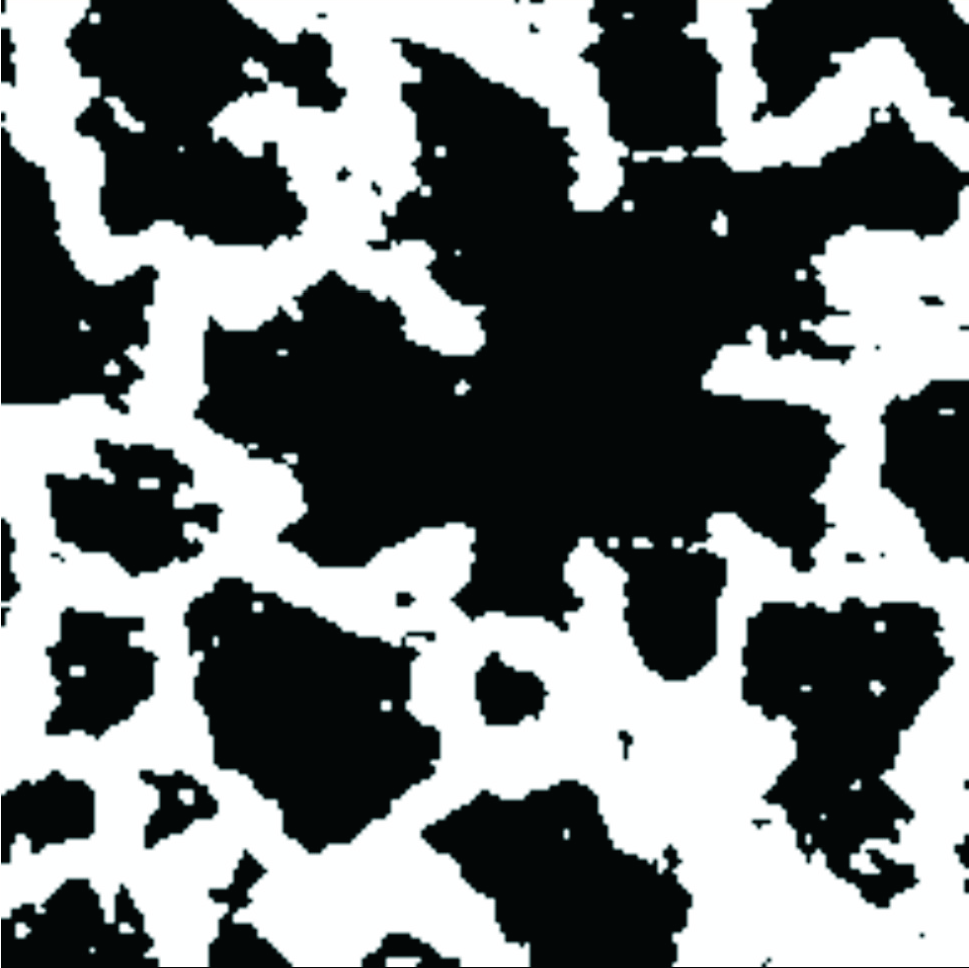
\includegraphics[width=\imsize]{img/Tsuda2008/Tsuda-06b}%
				\label{subfig:tsuda-06b}%
			}%
		}\hfill%
		\subfloat[]{%
			\fbox{%
				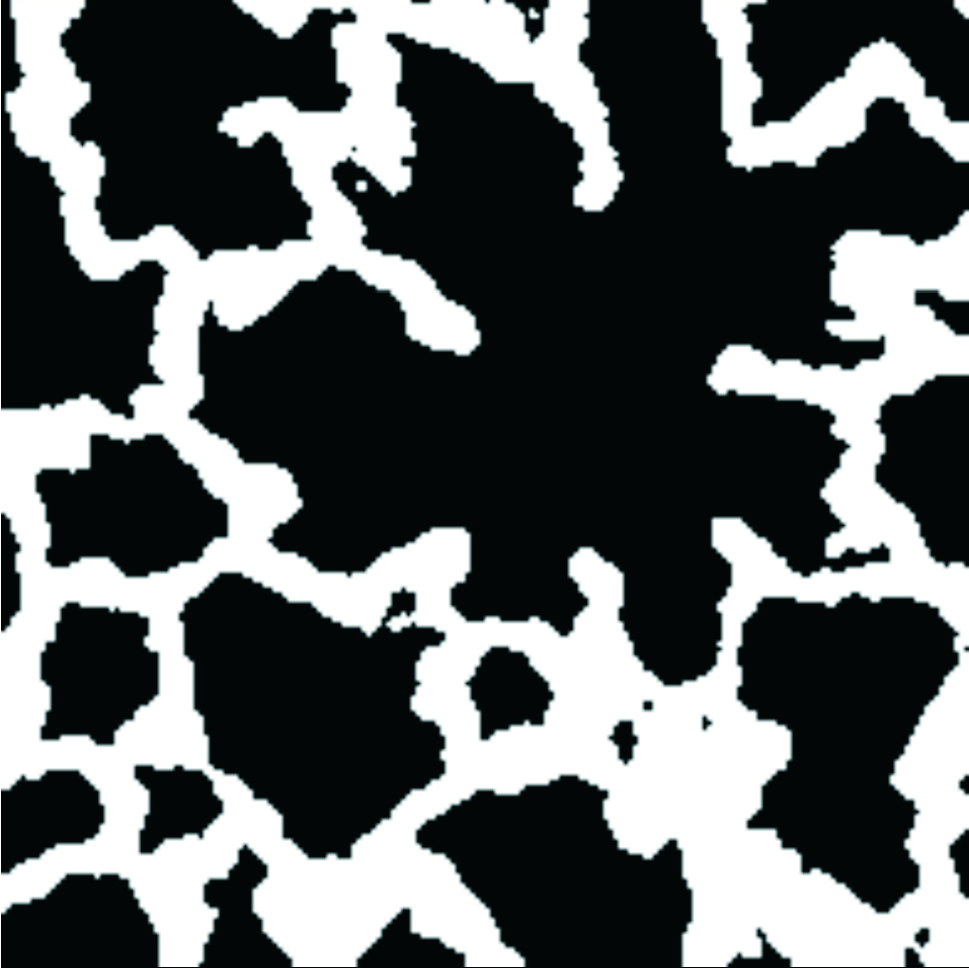
\includegraphics[width=\imsize]{img/Tsuda2008/Tsuda-06c}%
				\label{subfig:tsuda-06c}%
			}%
		}\hfill%
		\subfloat[]{%
			\fbox{%
				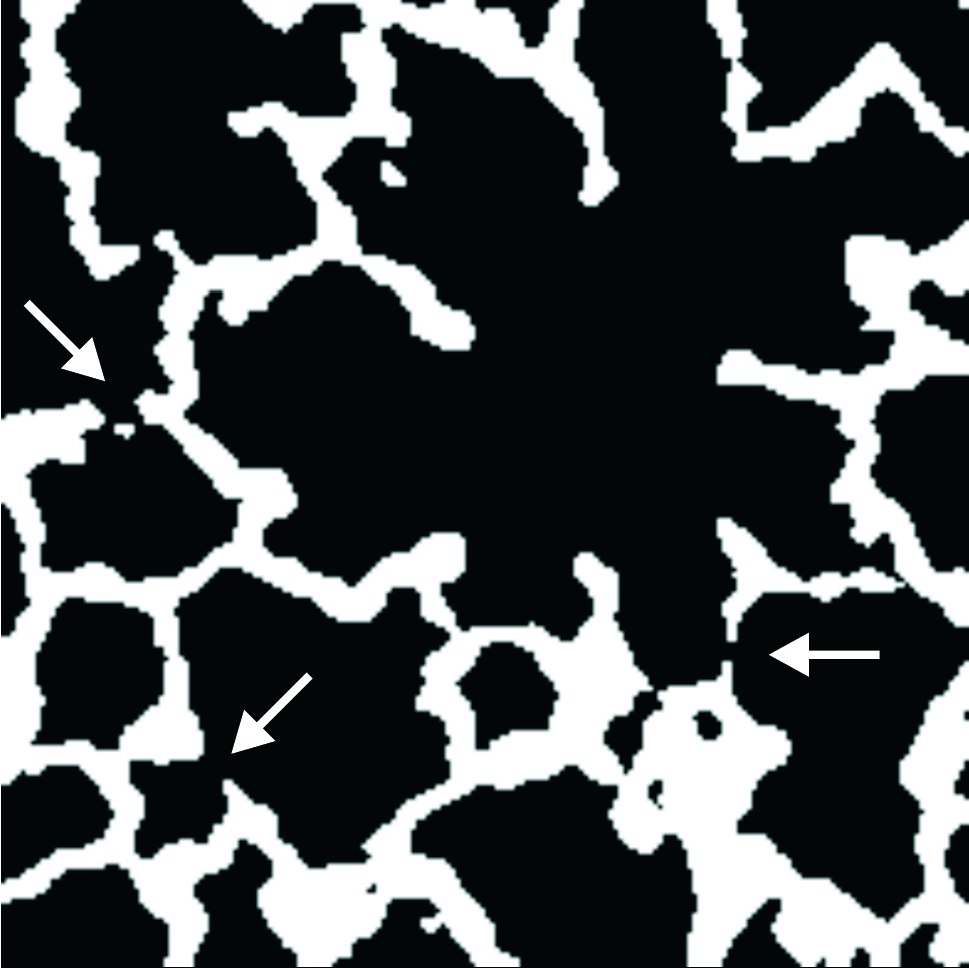
\includegraphics[width=\imsize]{img/Tsuda2008/Tsuda-06d}%
				\label{subfig:tsuda-06d}%
			}%
		}%
	}%
	\caption[Thresholding Influence]{\subref{subfig:tsuda-06a}: original slice from raw data. \subref{subfig:tsuda-06b}: thresholded with a value of 130, meaning that all pixels below 130 are set to black, all pixels with a value of 130 or greater are set to white. Resulting alveolar walls are too thick. \subref{subfig:tsuda-06c}: thresholded with a value of 139. Image looks correct. At this threshold the observed thickness of the septa was smaller than \SI{10}{\micro\meter}. In the same animals \cite{Roth2005} the thickness of the septa was determined as they appeared on electron microscopical images. They measured a mean of \SI{8}{\micro\meter}. \subref{subfig:tsuda-06d}: thresholded with a value of 148. Alveolar walls are too thin, and multiple erroneous holes (arrows) appear in the tissue.}
	\label{fig:tsuda-06}
\end{figure}

\subsection{FE \threed reconstruction}
Prior to the \threed reconstruction, the \ was performed to screen small objects with unreasonable size; voxels of those unreasonably small objects were reclassified to match the surrounding voxels. After successful preprocessing, \threed reconstruction was performed using \ac{gbha}. The examples with three different values of threshold level (130, 139, 148), corresponding to those in \autoref{fig:tsuda-06}, are shown in \autoref{fig:tsuda-07}. As is expected, the \threed reconstructed object appears to have thick tissue walls with the lower threshold value of 130, while it appears to be too thin, with many holes with the higher threshold value of 148. With the intermediate threshold value of 139, the structure appears to be reasonable. This will be tested quantitatively next.

\subsection{Validation of Segmentation and Image Processing}
To perform a statistical analysis for the selection of the threshold value, five pieces of parenchymal sample (200$\times$200$\times$180 pixels) were selected. We calculated the V\textsubscript{VS} of each \ac{roi} after the \threed reconstruction, and the average value with \ac{se} was plotted as a function of threshold level (\autoref{fig:VVSplot}). Our calculated value of V\textsubscript{VS} nearly linearly decreased with increasing threshold level and our V\textsubscript{VS} matches the gold standard value of 0.196 at a threshold value of 139. In addition, the values of calculated SE were generally very small, indicating that each sample, although small in size, represented typical parenchymal structure. We determined to use a threshold value of 139 for this tissue sample.

The surface area density of air space (S\textsubscript{VS} [\centimetresquared\per\centimetrecubed]) of each \ac{roi} sample was also calculated and plotted (\autoref{fig:VVSplot}). As we expected, however, S\textsubscript{VS} shows poor match with the reported value of \num[seperr]{904(84)}~(\acs{se}) over almost the entire range of threshold levels tested and especially at the threshold value of 139. The cause of this discrepancy will be discussed in detail in \autoref{sec:discussion}.

\renewcommand{\imsize}{0.47\linewidth}
\begin{figure}
	\noindent\makebox[\textwidth]{%
		\subfloat[]{%
			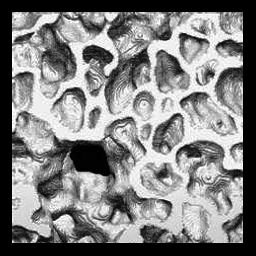
\includegraphics[width=\imsize]{img/Tsuda2008/Tsuda-07a}%
			\label{subfig:tsuda-07a}%
		}%
		\subfloat[]{%
			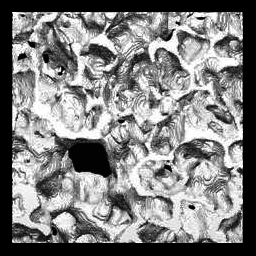
\includegraphics[width=\imsize]{img/Tsuda2008/Tsuda-07b}%
			\label{subfig:tsuda-07b}%
		}%
		\subfloat[]{%
			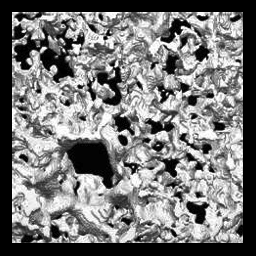
\includegraphics[width=\imsize]{img/Tsuda2008/Tsuda-07c}%
			\label{subfig:tsuda-07c}%
		}%
	}%
	\\%
	\noindent\makebox[\textwidth]{%
		\subfloat[]{%
			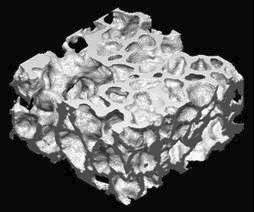
\includegraphics[width=\imsize]{img/Tsuda2008/Tsuda-07d}%
			\label{subfig:tsuda-07d}%
		}%
		\subfloat[]{%
			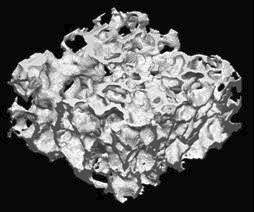
\includegraphics[width=\imsize]{img/Tsuda2008/Tsuda-07e}%
			\label{subfig:tsuda-07e}%
		}%
		\subfloat[]{%
			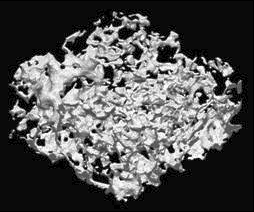
\includegraphics[width=\imsize]{img/Tsuda2008/Tsuda-07f}%
			\label{subfig:tsuda-07f}%
		}%
	}%
	\caption[Three-dimensional reconstruction of tissue]{Three-dimensional reconstruction of tissue. \subref{subfig:tsuda-07a} and \subref{subfig:tsuda-07d}: threshold 130. \subref{subfig:tsuda-07b} and \subref{subfig:tsuda-07e}: threshold 139. \subref{subfig:tsuda-07c} and \subref{subfig:tsuda-07f}: threshold 148.}
	\label{fig:tsuda-07}
\end{figure}

\renewcommand{\imsize}{\linewidth}
\begin{figure}
	\centering
	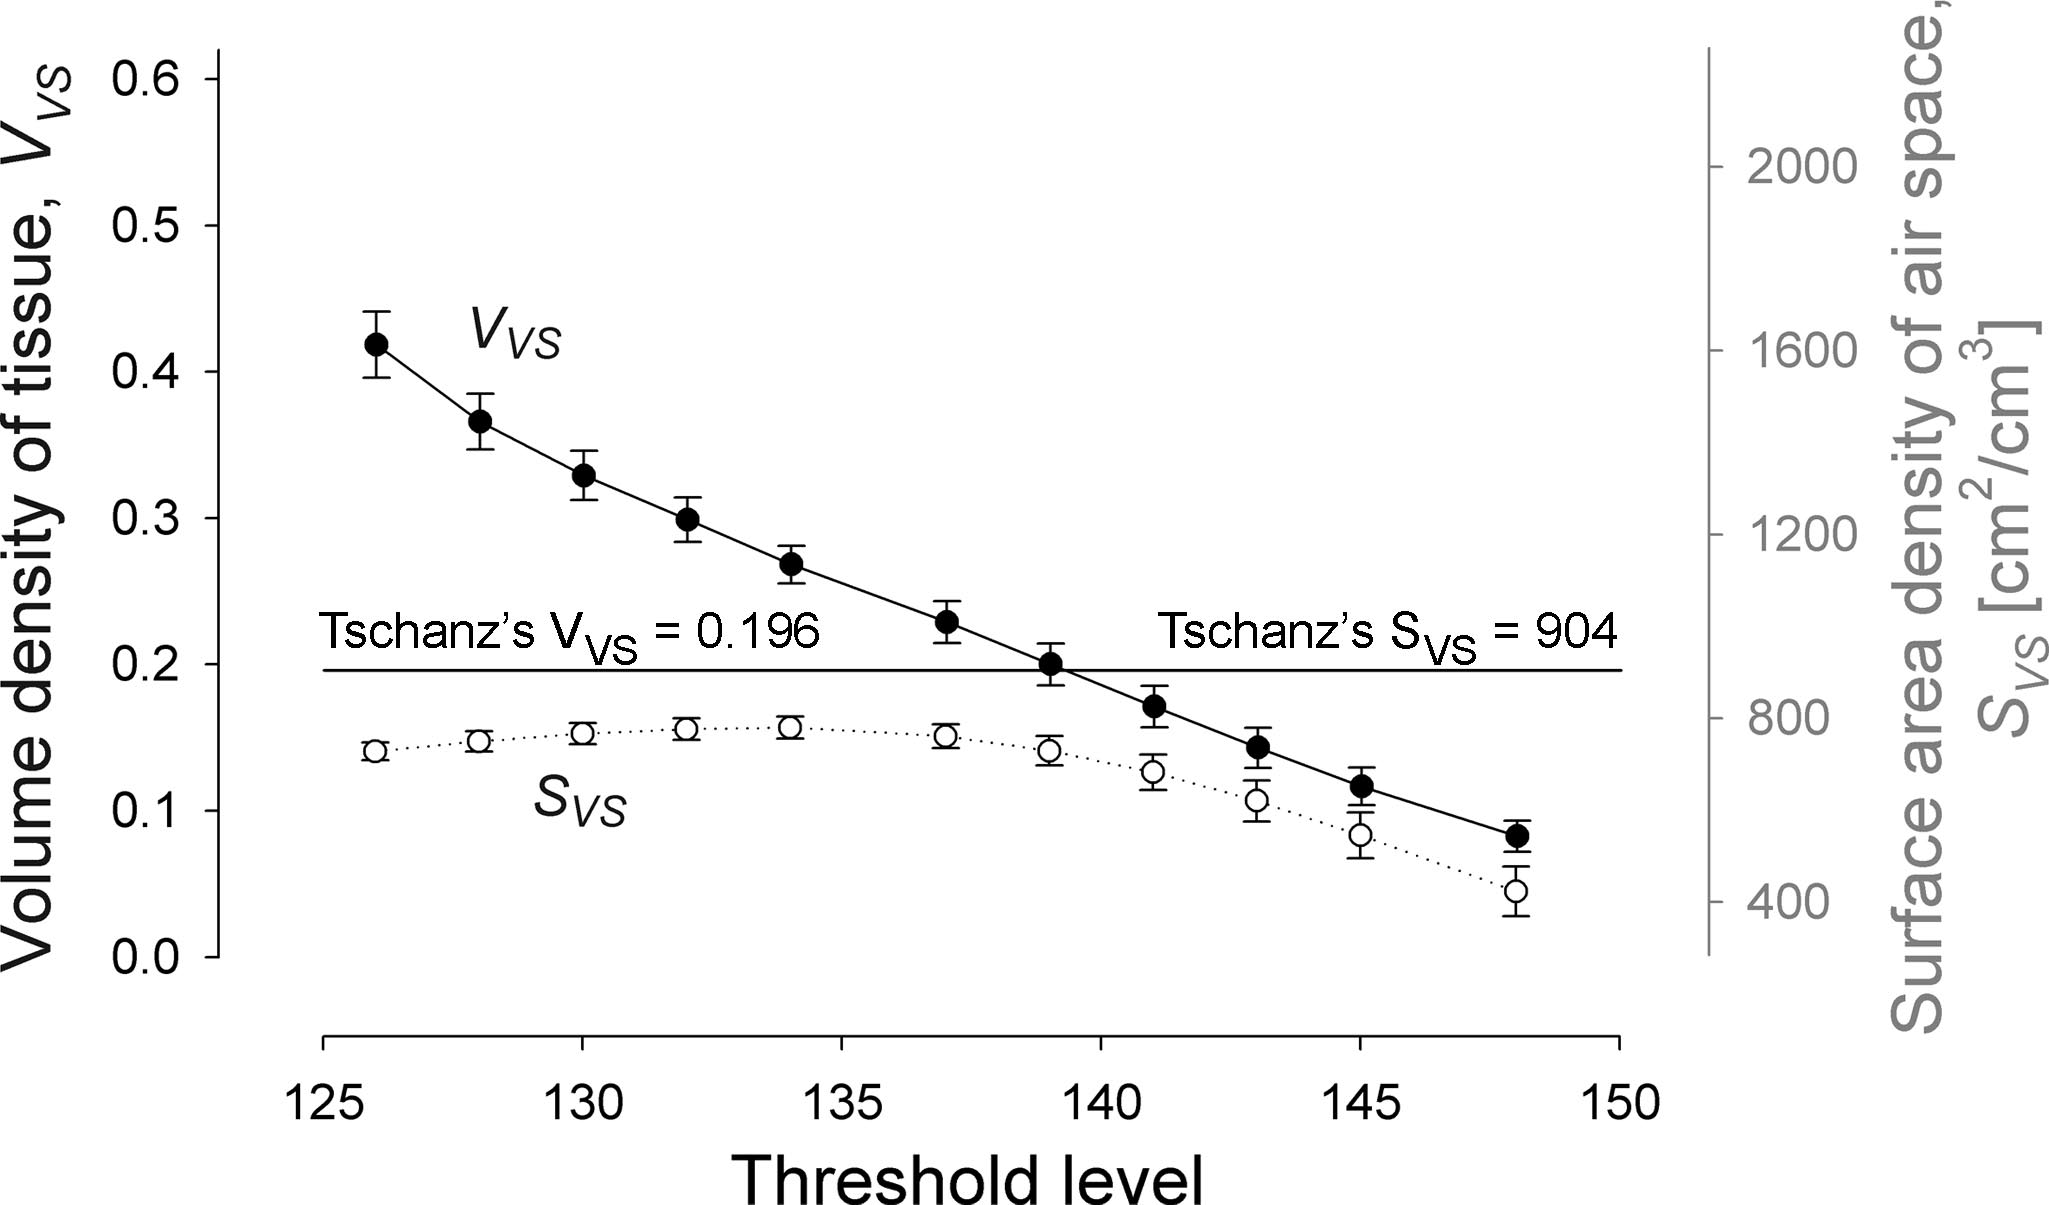
\includegraphics[width=\imsize]{img/Tsuda2008/Tsuda-08}
	\caption[Average volume density of tissue and surface area density of air space]{Average volume density of tissue (V\textsubscript{VS}) and surface area density of air space (S\textsubscript{VS}) of \acp{roi}, plotted as a function of threshold level. Error bars represent standard error. Our V\textsubscript{VS} matches the gold standard value of 0.196 at a threshold value of 139. Bars include the standard error, n=5.}
	\label{fig:VVSplot}
\end{figure}

\subsection{FE \threed Reconstruction of Air Space}
\threed air spaces, separated by tissues, in the \ac{roi} were also constructed (\autoref{fig:tsuda-09}). To demonstrate air space configuration more clearly, a small alveolated air section was isolated from the center of \ac{roi} and was enlarged in an inset of \autoref{fig:tsuda-09}. These \threed air objects packed with several million \threed 8-node \acp{fe} (a mixture of structured and unstructured cubic elements) can be readily used for \ac{fe} calculations, including airflow \ac{cfd}, in the future.

\section{Discussion}\label{sec:discussion}
We described our custom-made \ac{fe} methodology to reconstruct the acinar air space as well as septal tissue of rat lung in three dimensions. Approximately \SI{3}{\milli\meter\cubed} (=3$\times10^9$~\micro\meter$^3$) of fixed lung tissue was scanned with high resolution \ac{srxtm} (voxel size=\SI{1.4}{\micro\meter\cubed}) and a stack of 1024 image slices (1024$\times$1024~pixels) was prepared for \threed rendering. After preprocessing the raw voxel data with a tentative threshold level, \threed \acp{fe} were created overlaying the voxel map using a \ac{gbha}. A proper threshold value for adequate segmentation was iteratively determined to match the calculated volume density of tissue (V\textsubscript{VS}) to the stereological determined value \cite{Tschanz2003}. With the optimized algorithms (a combination of \ac{oca} and \ac{gbha} algorithms), \acsu{cpu} time for one iteration for $\sim$8 million voxels was $\sim$\SI{90}{\minute} by a standard \ac{pc}.

\subsection{Historical Perspective}
Acinar structure was traditionally studied using lung cast models \cite{Boyden1971,Haefeli1988,Schreider1981} or serial histological sections (\eg, \cite{Berend1991,Hansen1975,Hansen1975a,Parker1971,Randell1989}). With the former approach, some types of measures are not possible: only the polymer-filled air spaces are available for measurement as the tissue is digested away, and internal data are lost as scanning electron microscopy is limited to the exposed surfaces of the cast. \threed rendering of alveolar geometries from histological sections requires careful, time-consuming alignment and registration of serial \twod sections \cite{Mercer1987,Mercer1987a,Stelter1966}, which generally limits reconstruction to just a few alveoli~\cite{Mercer1987}. An additional drawback is sample destruction and deformation from physical sectioning.

Optical sectioning permits faster, less invasive, more thorough digital analysis and \threed rendering than is possible with physical sectioning. Large upper airways can be analyzed with modern techniques such as magnetic resonance microscopy~\cite{Hoffman1990,Sundaramoorthy1995} or optical coherence tomography~\cite{Hanna2005}; functional imaging of the lung by \ac{ct} and \ac{mri} has recently been summarized by \citet{VanBeek2008}. Laser scanning confocal microscopy provides sufficient resolution to image fine-scale acinar detail, but there have been very few \threed acinar reconstruction studies using this method. \citet{Cookson1993} used serial optical sections acquired by confocal microscopy to produce \threed volume renderings of human alveolar ducts. This approach is restricted in that imaging depth below the tissue surface is limited by light penetration and the working distance of the objective lens~\cite{Bonse1996}. \citet{Cookson1993} warned that caution was necessary in interpreting confocal \threed renderings because the relative contributions of the various factors (refractive index changes, tissue density changes, resorption) causing depth-dependent loss of resolution and/or intensity were difficult to measure and correct. Multiphoton microscopy improves imaging depth, but the imaging depth is still restricted to $\sim$\SI{100}{\micro\meter} into the lung \cite{Pena2007}. For comparison, human alveolar ducts range from 270 to \SI{600}{\micro\meter} in diameter \cite{Whimster1970}. Thus sample size constraints limit confocal analysis to just a small portion of the acinus, restricting its usefulness in studies of flow and aerosol particle deposition. In the early 1990s, new imaging techniques, such as \ac{ct} \cite{Brown1991,Mcnamara1992}, permitted measurement and reconstruction of the \threed structure of the bronchial tree and small airways \cite{Aykac2003,Higgins1998,Park1998,Reinhardt1997,Sauret2002,Sera2003,Wood1995,Wood1995a}. Successful visualization of the acinar region, though, was limited by the spatial resolution of standard \ac{uct}. In the past few years, however, \ac{uct}-based \threed reconstruction and morphometric analysis of the alveolar region has become possible \cite{Langheinrich2004,Litzlbauer2006,Watz2005}, facilitated by the advent of \ac{srct}. \ac{srct} is to be distinguished from \ac{srxtm} \cite{Schittny2008,Stampanoni2002,Stampanoni2007}. While during \ac{srct} the X-rays are directly recorded after transmitting the sample, during \ac{srxtm} the transmitted images are first recorded on a scintillator and magnified 5--20 times by a light microscope before recording.

\subsection{srxtm}
\ac{sr} is an electromagnetic wave emitted from electrons traveling near the speed of light when their path is bent by a magnetic field \cite{Iida2003}. A synchrotron facility is an excellent source of the most useful electromagnetic waves to explore materials and biological systems: X-ray ultraviolet and infrared light. Here we limit our discussion particularly to the application of \ac{sr} for X-ray tomographic microscopy (\autoref{fig:imaging setup}) highlighting the following superb features.

\renewcommand{\imsize}{0.705\linewidth}
\begin{figure}
	\noindent\makebox[\textwidth]{%
		\subfloat[]{%
			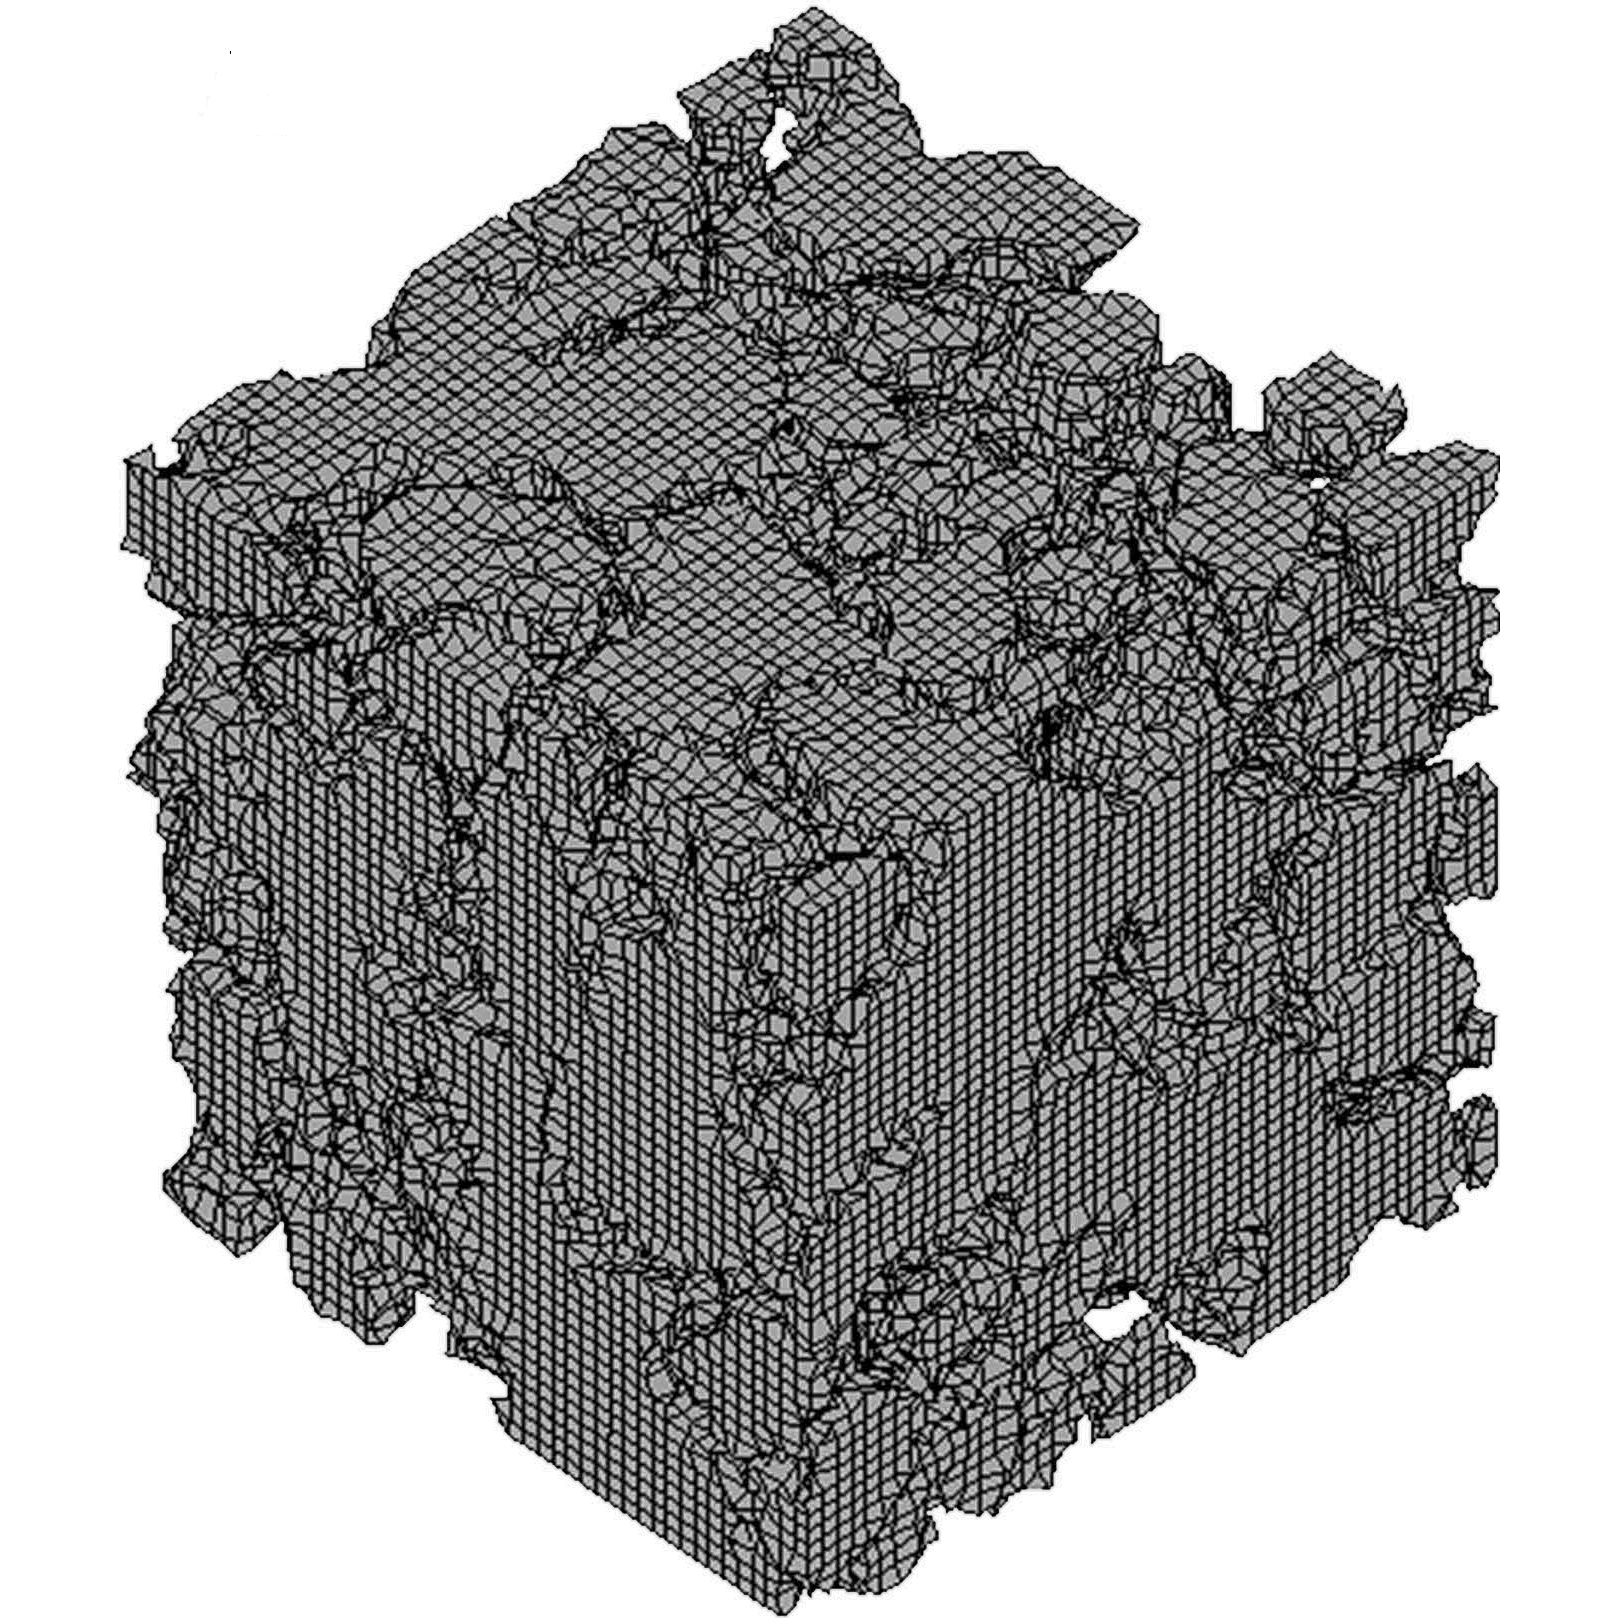
\includegraphics[width=\imsize]{img/Tsuda2008/Tsuda-09a}%
			\label{subfig:tsuda-09a}%
		}\hfill%
		\subfloat[]{%
			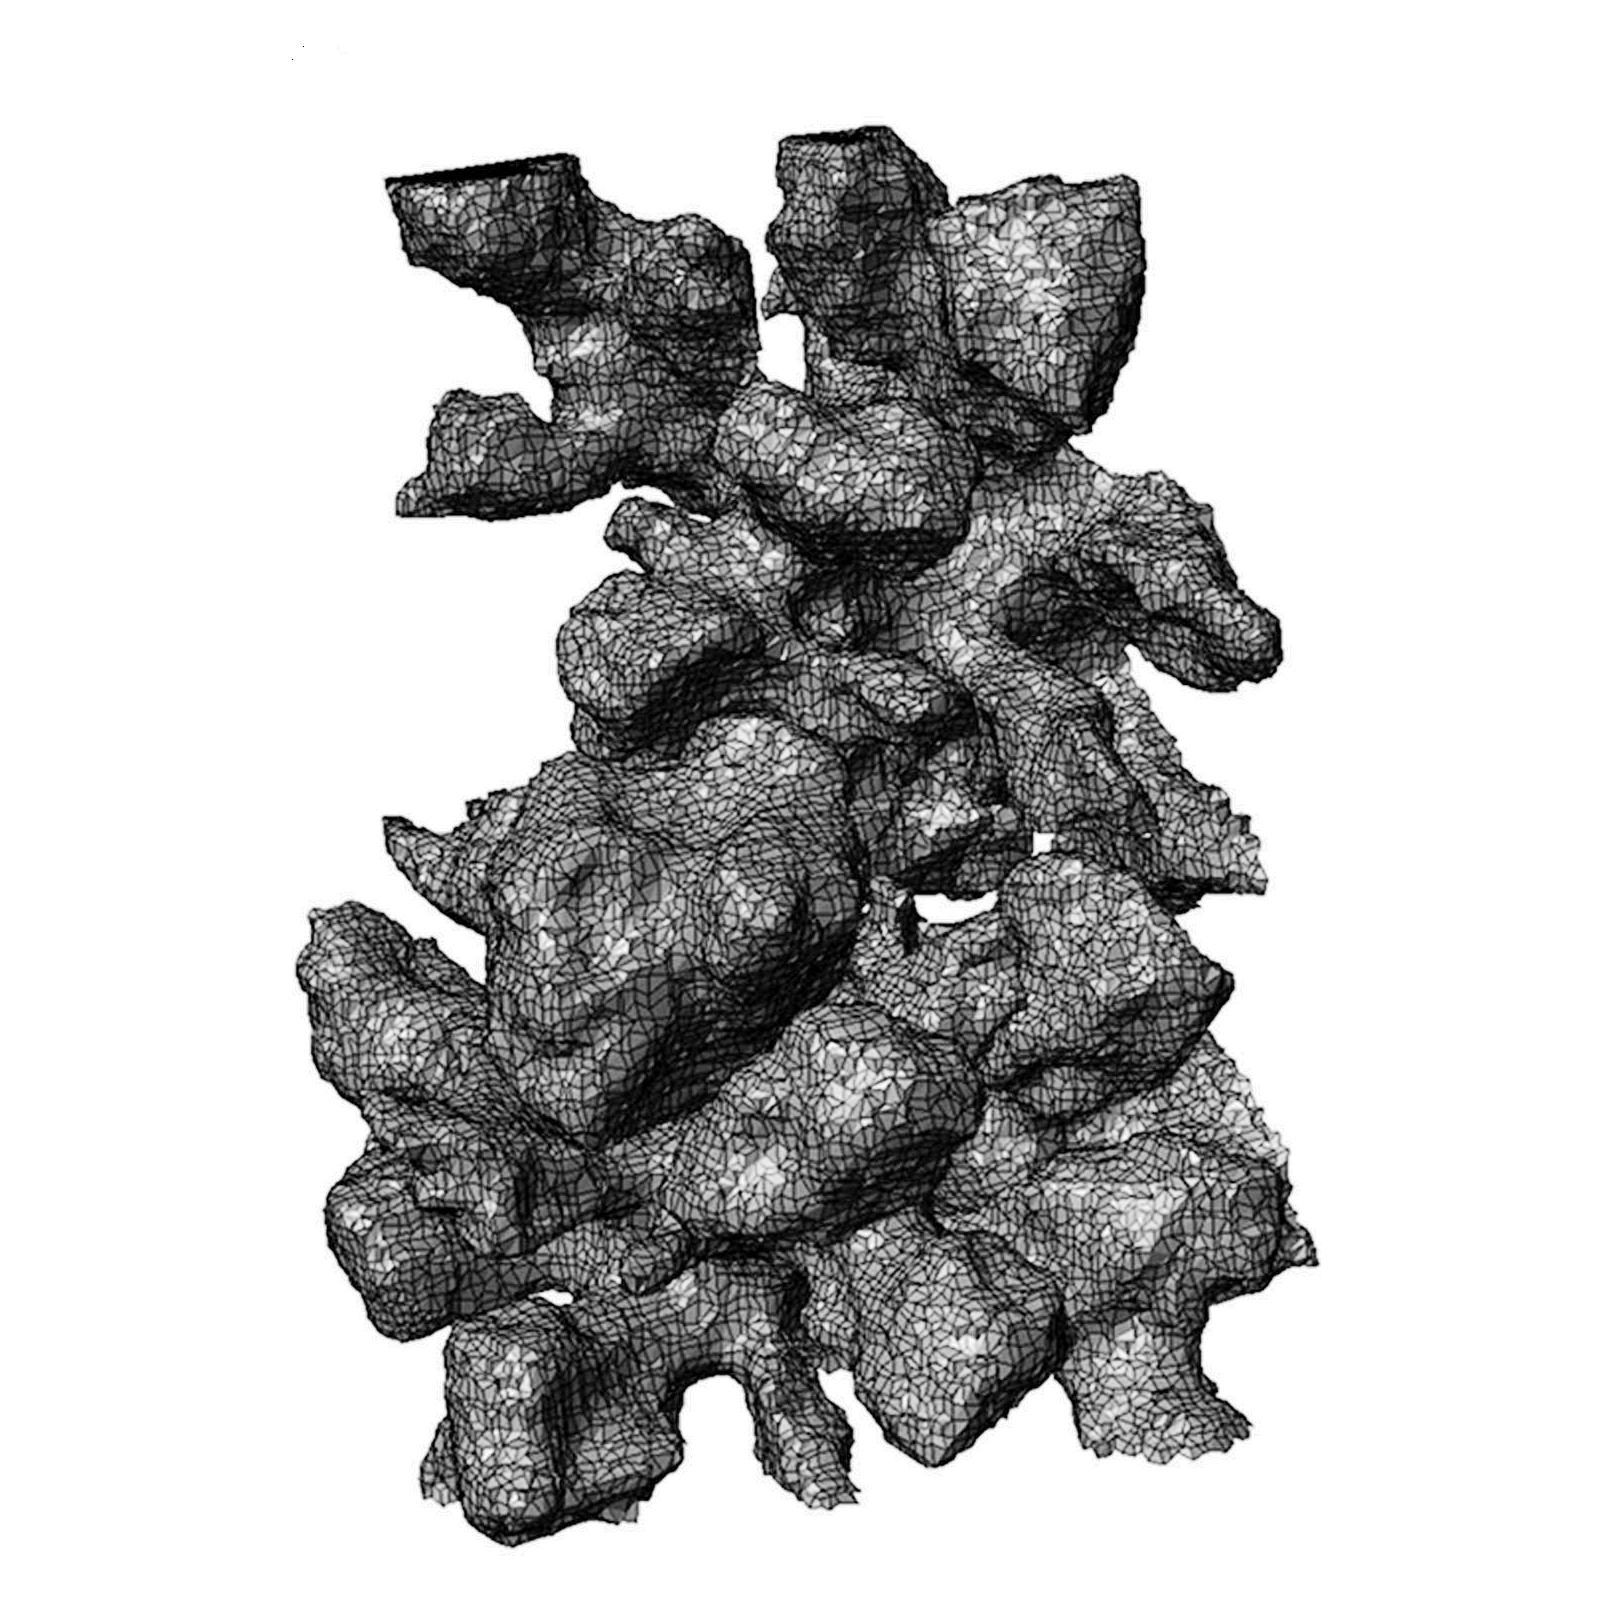
\includegraphics[width=\imsize]{img/Tsuda2008/Tsuda-09b}%
			\label{subfig:tsuda-09b}%
		}%
	}%
	\caption[Three-dimensional reconstruction of air spaces]{\subref{subfig:tsuda-09a}: reconstruction of \threed air spaces separated by tissues from \ac{roi}. \subref{subfig:tsuda-09b}: enlargement of a small alveolated air section isolated from the center of the \ac{roi}.}
	\label{fig:tsuda-09}
\end{figure}

\subsubsection{High power and high brilliance}
\ac{sr} is extremely powerful but even more important is that this radiation is emitted by a small source area and that this emission occurs within a narrow angular cone. Bending magnets or sophisticated insertion devices (called undulators or wigglers) produces therefore a high brilliant radiation that is several orders of magnitude more bright than conventional X-ray tubes (\autoref{fig:imaging setup}). This makes the usage of monochromators\graffito{A monochromator is a device in X-ray optics that is used to select a defined wavelength of the radiation for further use in a dedicated instrument or beamline.} particularly interesting since an extremely intense photon flux at a selected energy (or wavelength) can easily be extracted from the white beam emitted by the source (\autoref{fig:imaging setup}). The X-ray energy can be adjusted ``ad hoc'' to the sample, according to its absorption properties. The monochromaticity of the beam is an important feature of \ac{sr} application, critical for tomography applications since it automatically eliminates beam hardening artifacts from the tomographic reconstruction.

The high collimation of the \ac{sr} produces ``de facto'' a parallel beam at the sample location: the resulting negligible geometrical blur makes it possible to obtain images with high spatial resolution and a high \ac{snr}. Since, for a given \ac{snr} and a given contrast, the necessary photon flux scales with the fourth power of the spatial resolution \cite{Bonse1996} it is obvious that \ac{sr}-based tomography is perfectly suited for investigations with spatial resolution in the micrometer or even submicrometer range. Nowadays, X-ray tomographic microscopy endstations installed at third generation synchrotron facilities like \ac{tomcat}~\cite{Stampanoni2007} routinely reach resolution $\sim$\SI{1}{\micro\meter} within scan times of a few minutes.

Synchrotron radiation-based \ac{ct} overcomes the critical technical issue (resolution) that has prevented fine-scale structural analysis of the acinus by tabletop X-ray \ac{uct}. The brilliant, highly collimated beam provides a nearly ideal X-ray source for \ac{uct}~\cite{Jorgensen1998}, producing greater spatial resolution. This allows high-resolution imaging of unprocessed lung tissue \cite{Bayat2006,Jheon2006,Monfraix2005,Sera2007,Sera2005} and ultra high resolution (from $<$1 to \SI{15}{\micro\meter}, with tissue thicknesses of $\geq$\SI{1500}{\micro\meter}) visualization and \threed reconstruction of small airways and alveoli in processed tissue \cite{Ikura2004,Schittny2008}.

\subsection{Segmentation/Threshold}
Careful determination of the proper threshold level is essential for accurate \threed rendering and for the first step of \ac{fe}-mesh generation. If the level is too low, the fraction of air would become unrealistically small relative to tissue resulting in thicker septa. If the level is too high, on the other hand, the fraction of air becomes unrealistically large relative to tissue; thinner tissue would result in artificial holes in the septal walls or even too many unconnected tissue pieces in the sample. This would have a direct impact on the skeletonization process (which is not dealt with in this paper), as well as the subsequent \ac{fe} analyses, such as airflow simulations. Our \ac{oca} is designed to minimize this problem.

A unique aspect of our work is that segmentation was done iteratively by searching for the optimal threshold value (\autoref{fig:workflow}). In every iteration, the key morphological parameter (discussed below in detail) was calculated and compared with the gold standard; the iteration was continued until the calculated value matched the gold standard. This gold standard was previously determined in the tissue sample from exactly the same animal~\cite{Tschanz2003}. Because our main aim in this work was to develop \ac{fe} methodology, this selection of tissue sample, whose morphology has been thoroughly analyzed, is very well suited for this project.

The key morphological parameter we tried to match was the volume density of tissue (V\textsubscript{VS}). The V\textsubscript{VS} is an easy to calculate parameter (\ie, the sum of \ac{fe} volume belonging to tissue divided by the sum of all \ac{fe} volume) and is relatively insensitive to the resolution of the measurement technique. The calculated V\textsubscript{VS} decreases almost linearly with an increase in the threshold level (\ie, a fraction of air volume relative to tissue volume) around the gold standard value (V\textsubscript{VS}=0.196 in our case, see \autoref{fig:VVSplot}). At the threshold value of 139, the calculated V\textsubscript{VS} was within \SI{2}{\percent} difference of the gold standard.

\renewcommand{\imsize}{\linewidth}
\begin{figure}
	\centering
	\pgfmathsetlength{\imagewidth}{\imsize}%
	\pgfmathsetlength{\imagescale}{\imagewidth/1500}%
	\def\x{927}%
	\def\y{800}% scalebar-y at 90% of height of y=1715px
	\begin{tikzpicture}[x=\imagescale,y=-\imagescale]
		\node[anchor=north west,inner sep=0pt,outer sep=0pt] at (0,0) {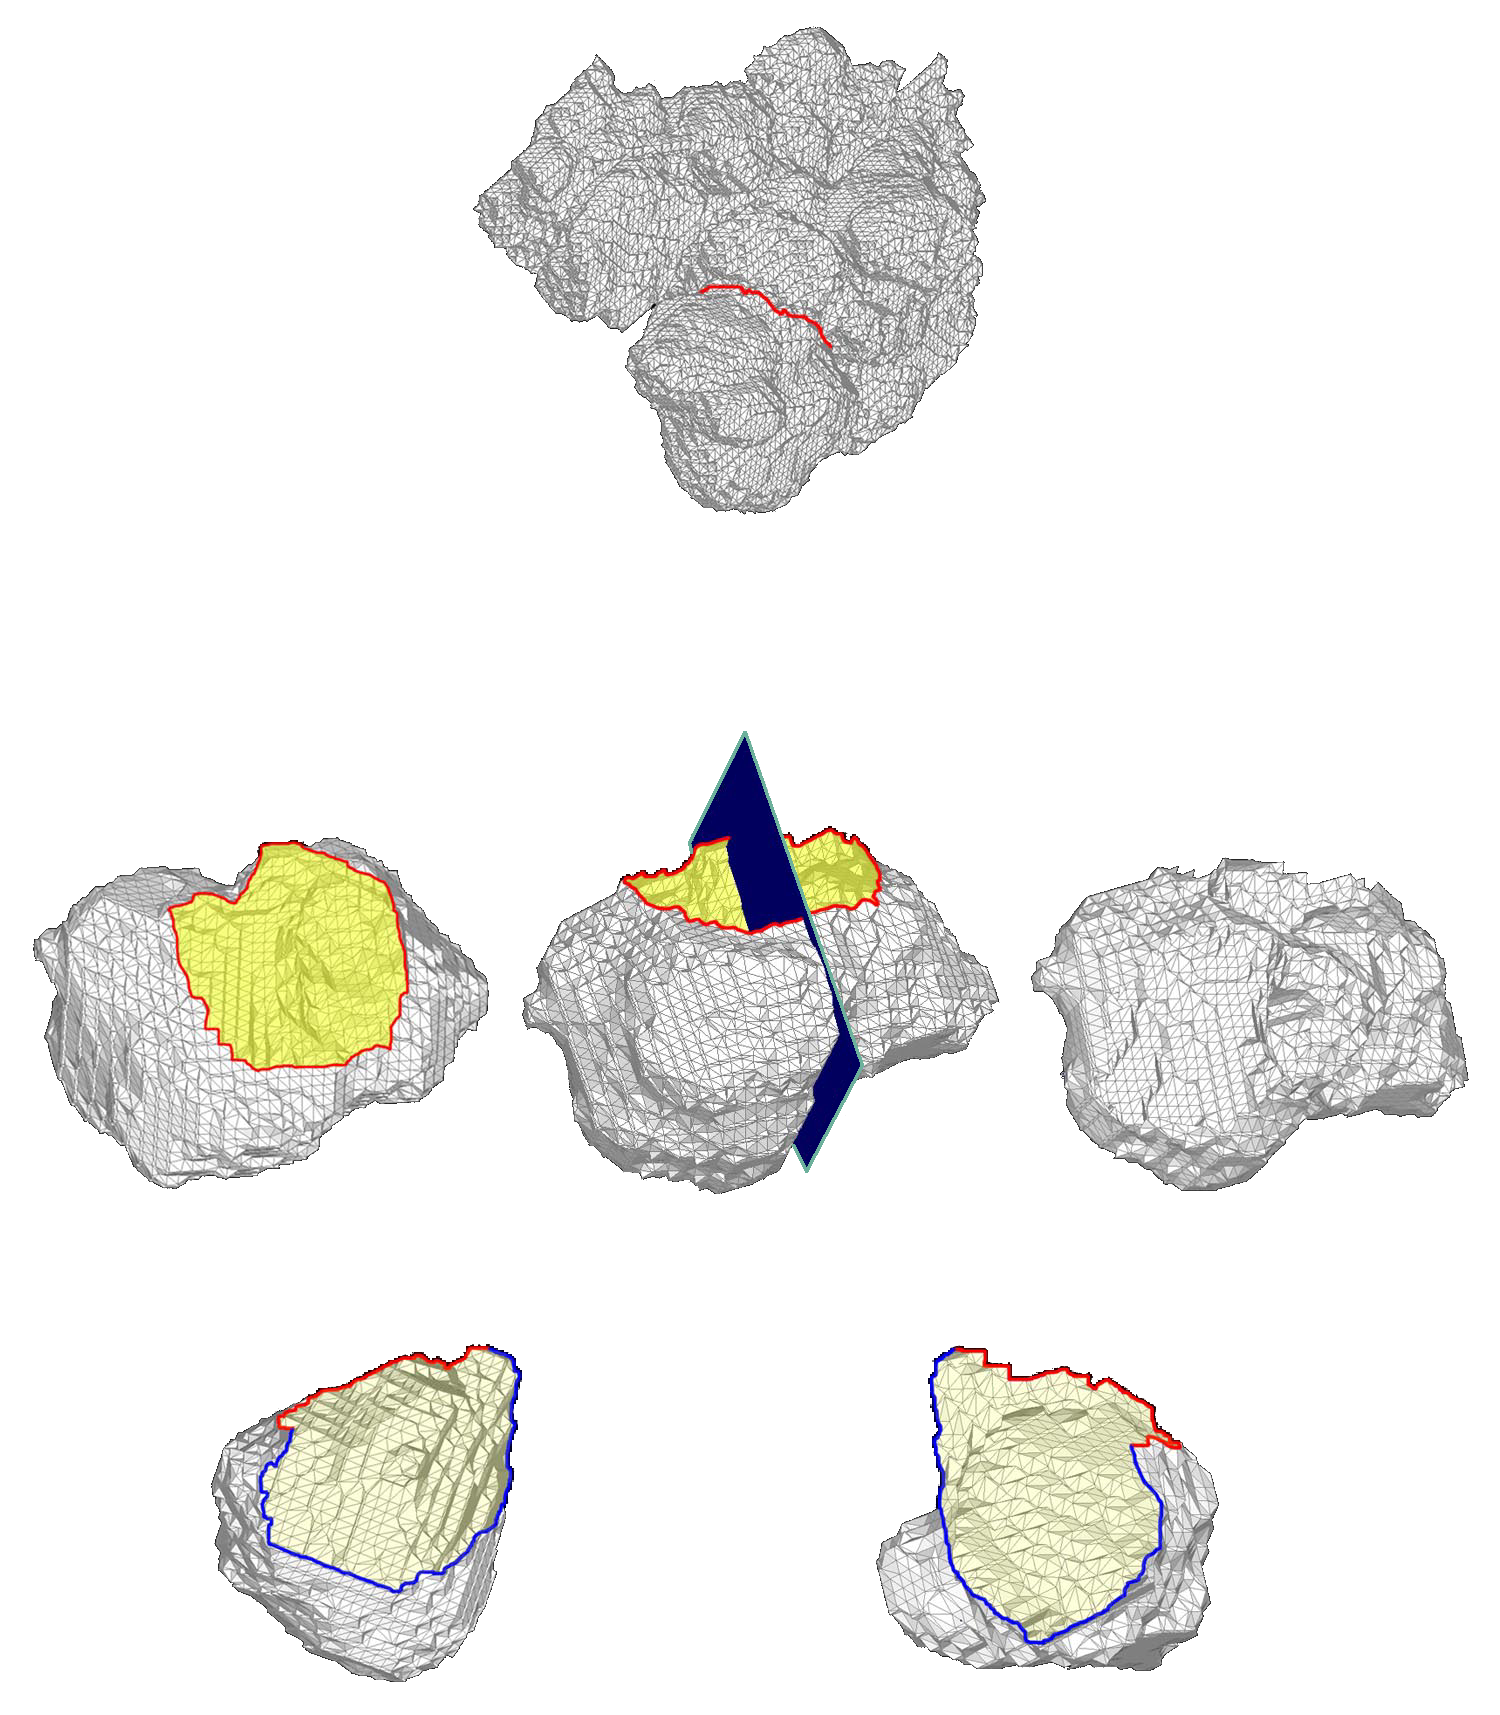
\includegraphics[width=\imagewidth]{img/Tsuda2008/Tsuda-10_edit}};
		% 95px = 0.01mm > 100px = 11um > 4752px = 500um, 950px = 100um
		%\draw[red,|-|,thick] (881,1100) -- (976,1100) node [sloped,midway,above] {\SI{0.01}{\milli\meter} (100px)};
		\draw[|-|,thick] (\x-47.5,\y) -- (\x+95,\y) node [midway, above] {\SI{10}{\micro\meter}};
		\draw[->,thick] (750,540) -- (750,690);%length of 150
		\def\a{106.06601717798212866012665431573}%=sin(45)*150
		\draw[->,thick] (825,1220) -- (825+\a,1220+\a);
		\draw[->,thick] (675,1220) -- (675-\a,1220+\a);
	\end{tikzpicture}%
	\caption[Three-dimensional \acs{fe} shell model of a partial acinus]{Three-dimensional \ac{fe} shell model of acinus viewed from different angles. Top: \ac{roi}. Middle: top view (\textit{left}); side view (\textit{middle}); bottom view (\textit{right}). Bottom: alveolar inside views.}
	\label{fig:alveolus}
\end{figure}

We also calculated surface area density of air space (S\textsubscript{VS} [\centimetresquared\per\centimetrecubed]) and compared it with the value reported by \cite{Tschanz2003}. However, our calculated values were always lower than the reported value (S\textsubscript{VS}=904 [\centimetresquared\per\centimetrecubed]). This is because although the volume is relatively insensitive to the resolution of the measurement technique, the air-tissue boundary (surface area) is highly sensitive to how it is measured. S\textsubscript{VS} reported in \citet{Tschanz2003} was measured at a $\times$10 secondary magnification after recording the electron microscopical images at a primary magnification of $\times$1200 on a \SI{35}{\milli\meter} film (theoretical resolution of $\sim$\SI{70}{\nano\meter}), while the resolution of our \threed reconstruction is \SI{1.4}{\micro\meter}. The extent of surface complexity is recognized differently, depending on the resolution of the measuring instrument; the finer the resolution of the sample and the instrument, the more surface detail can be detected. This is similar to the problem when one measures the length of the British coastline with different yardsticks~\cite{Mandelbrot1967}.

\subsection{\twod vs. \threed}
Morphological analyses in \threed are qualitatively different from stereology, which is an analysis made in \twod sections to infer \threed structure and morphometry. Apart from the most common measures of geometric/topological properties, such as the volume density, the area density, and the length density, stereological analysis is generally limited. For example, number density cannot be estimated stereologically using single sections without a significant number of a priori assumptions about the shape of the objects, including the question of whether the objects are convex and whether they are simply connected. These significant restrictions in the stereological analysis are due to the fact that it is based on the following two fundamental assumptions: 
\begin{enumerate}
	\item the structure is homogeneously distributed (\ie, spatially invariant) and 
	\item isotropically distributed (\ie, rotation invariant) in the tissue sample (J. P. Butler, personal communication). 
\end{enumerate}
The \threed analysis relaxes these restrictions either by going to full unrestricted \threed (\ac{uct}, \ac{mri}, \ac{srxtm}, etc.) or using two consecutive sections (disector) for the counting of numbers~\cite{Hyde2007}.

In addition to these fundamental differences, \threed analyses have numerous advantages over traditional stereology. The most obvious advantage is the flexibility of the analysis. It is often difficult to properly select a \ac{roi} because the exact location of the target region cannot be identified beforehand and in the traditional approach, one has only one opportunity to section the tissue sample. In the case of \threed reconstruction analysis, on the other hand, the selection of the \ac{roi} can be repeated as many times as required and the selection can be iteratively improved until the target \ac{roi} is obtained. Once the \ac{roi} is selected in \threed (\autoref{fig:alveolus}, \textit{top}), the target region (\eg, an alveolus) can be viewed from any arbitrary angle (see \autoref{fig:alveolus}, \textit{middle}), including from behind the object (\autoref{fig:alveolus}, \textit{middle right}), something not easily achievable otherwise. The \threed object can be cut into half (\autoref{fig:alveolus}, \textit{bottom}) and also be sliced to make \twod sections in any orientation with any slab thickness (data not shown) and there is no limitation in repeating the sectioning process. Furthermore, since the \ac{roi} can be viewed in any chosen angle and an internal view is possible, it is possible to fly through the structure to gain an internal view of the conduit once the \threed reconstructed structure is electronically available.

\subsection{FE \threed Rendering}
It is important to make a clear distinction between our \ac{fe} \threed rendering approach and the traditional surface triangulation approach that is most common in medical imaging software. The triangulation approach is mainly used for surface visualization; this uses a variety of filtering methods and surface smoothing techniques, but does not involve real volume like with our \ac{fe} \threed rendering method. If the volume compartment of either air or tissue is needed for subsequent analysis, such as for a calculation of fluid flow in acinar air space, a traditional surface triangulation approach does not provide a readily usable \threed structure; a volume bounded by the visualized surface needs to be further elementalized. Since we are in possession of a closed workflow for the further processing of the meshed surfaces (\ie, there is a single process from mesh generation through to visualization), intermediate conversions of the dataset into other formats are not required. This eliminates overhead and speeds the overall process. The \ac{fe} mesh of the data makes it possible to use it for volume rendering, further processing (with the use of quasi-standard \acs{stl} file format\graffito{An \acs{stl} file describes a raw unstructured triangulated surface by the unit normal and vertices of the triangles using a \threed Cartesian coordinate system.}), and direct import into the software used for \ac{cfd} calculations and evaluation of morphological factors. Since we also obtain a mesh inside the structure, we lay the groundwork for the skeletonization (extraction of the mean middle line) of the terminal airways and the determination of the entrance ring of a single alveolus.

The main aim of this project is a direct elementalization of air (or tissue) space using \ac{fe} technique. By isolating air (or tissue) from the rest (tissue or air, respectively), the interface of these two volume components, \ie, an air-tissue barrier, is automatically identified. For this isolation, we adapted the \ac{gbha} proposed by \citet{Schneiders1996}. First, an \ac{fe} mesh was overlaid on the voxel map. Basically, a relation of one \ac{fe} to one voxel could be used, but one practical problem may arise. That is, if the number of voxels in the original data is too large (i.e., in an order of billion in the case of our raw data) for a common \ac{pc} to handle easily, we may need to reduce the number ratio between \ac{fe} and voxel. The important points to achieve are, generally, 
\begin{enumerate}
	\item to reduce the number of \acp{fe} to a reasonable number but
	\item to still produce a smooth surface boundary.
\end{enumerate}
We use hexahedral \ac{fe} for this. An air-tissue interface was smoothed by adjusting the locations of \ac{fe} nodal points near the interface based on their original grayscale pixel intensity values. The distortions of \ac{fe} elements, if this happened as a result of the initial nodal relocation, were corrected and refined (see \autoref{sec:methods} for details). The resulting \threed \ac{fe} mesh (\eg, Figures~\ref{fig:tsuda-09} and \ref{fig:alveolus}) demonstrates reasonable acinar volume rendering.

Finally, for the type of image analysis discussed in this paper, the need for massive computation for \threed rendering as well as subsequent \ac{fe} computational analyses is unavoidable. In this regard, improving our computational capability, particularly by using parallel and grid computing algorithms, would be required in the near future.

\section{Acknowledgments}
We thank F. Marone and C. Hintermüller (Swiss Light Source, Paul Scherrer Institute) for expert help at the Beamline; B.\ de Breuyin, K.\ Sala-Szymanska, and B.\ Haenni for the embedding and preparation of the samples; C.\ Lehmann for the tricky shaping of the samples on the lathe; and D.\ Petrovic for preparing \autoref{fig:alveolus}. We also thank J.\ P.\ Butler and S.\ Tschanz for useful discussion on the subject of stereology.

This work was supported by National Heart, Lung, and Blood Institute Grants HL-054885, HL-070542, and HL-074022, Serbian Ministry of Science, OI144028, TR12007, and Swiss National Science Foundation Grant 3100A0-109874/1.
%\bibliographystyle{plainnat}
%\label{app:bibliography} 
%\bibliography{../Bibliography,../../references,../Tsuda2008references}